%% Based on a TeXnicCenter-Template by Tino Weinkauf.
%%%%%%%%%%%%%%%%%%%%%%%%%%%%%%%%%%%%%%%%%%%%%%%%%%%%%%%%%%%%%


%%%%%%%%%%%%%%%%%%%%%%%%%%%%%%%%%%%%%%%%%%%%%%%%%%%%%%%%%%%%%
%% HEADER
%%%%%%%%%%%%%%%%%%%%%%%%%%%%%%%%%%%%%%%%%%%%%%%%%%%%%%%%%%%%%
\documentclass[a4paper,oneside,10pt]{report}
% Alternative Options:
%	Paper Size: a4paper / a5paper / b5paper / letterpaper / legalpaper / executivepaper
% Duplex: oneside / twoside
% Base Font Size: 10pt / 11pt / 12pt


%% Language %%%%%%%%%%%%%%%%%%%%%%%%%%%%%%%%%%%%%%%%%%%%%%%%%
\usepackage[USenglish]{babel} %francais, polish, spanish, ...
\usepackage[T1]{fontenc}
\usepackage[ansinew]{inputenc}
\usepackage{caption} % for placing pictures not floating
\usepackage{lmodern} %Type1-font for non-english texts and characters
\usepackage{tikz}

\usepackage{listings}
%% Packages for Graphics & Figures %%%%%%%%%%%%%%%%%%%%%%%%%%
\usepackage{graphicx} %%For loading graphic files
%\usepackage{subfig} %%Subfigures inside a figure
%\usepackage{pst-all} %%PSTricks - not useable with pdfLaTeX

%% Please note:
%% Images can be included using \includegraphics{Dateiname}
%% resp. using the dialog in the Insert menu.
%% 
%% The mode "LaTeX => PDF" allows the following formats:
%%   .jpg  .png  .pdf  .mps
%% 
%% The modes "LaTeX => DVI", "LaTeX => PS" und "LaTeX => PS => PDF"
%% allow the following formats:
%%   .eps  .ps  .bmp  .pict  .pntg



%% Math Packages %%%%%%%%%%%%%%%%%%%%%%%%%%%%%%%%%%%%%%%%%%%%
\usepackage{amsmath}
\usepackage{amsthm}
\usepackage{amsfonts}


%% Line Spacing %%%%%%%%%%%%%%%%%%%%%%%%%%%%%%%%%%%%%%%%%%%%%
%\usepackage{setspace}
%\singlespacing        %% 1-spacing (default)
%\onehalfspacing       %% 1,5-spacing
%\doublespacing        %% 2-spacing


%% Other Packages %%%%%%%%%%%%%%%%%%%%%%%%%%%%%%%%%%%%%%%%%%%
%\usepackage{a4wide} %%Smaller margins = more text per page.
%\usepackage{fancyhdr} %%Fancy headings
%\usepackage{longtable} %%For tables, that exceed one page


%%%%%%%%%%%%%%%%%%%%%%%%%%%%%%%%%%%%%%%%%%%%%%%%%%%%%%%%%%%%%
%% Remarks
%%%%%%%%%%%%%%%%%%%%%%%%%%%%%%%%%%%%%%%%%%%%%%%%%%%%%%%%%%%%%
%
% TODO:
% 1. Edit the used packages and their options (see above).
% 2. If you want, add a BibTeX-File to the project
%    (e.g., 'literature.bib').
% 3. Happy TeXing!
%
%%%%%%%%%%%%%%%%%%%%%%%%%%%%%%%%%%%%%%%%%%%%%%%%%%%%%%%%%%%%%

%%%%%%%%%%%%%%%%%%%%%%%%%%%%%%%%%%%%%%%%%%%%%%%%%%%%%%%%%%%%%
%% Options / Modifications
%%%%%%%%%%%%%%%%%%%%%%%%%%%%%%%%%%%%%%%%%%%%%%%%%%%%%%%%%%%%%

%\input{options} %You need a file 'options.tex' for this
%% ==> TeXnicCenter supplies some possible option files
%% ==> with its templates (File | New from Template...).


% Theorems
\newtheorem{theorem}{Theorem}[section]
\newtheorem{corollary}[theorem]{Corollary}
\newtheorem{lemma}[theorem]{Lemma}
\newtheorem{definition}[theorem]{Definition}
\newtheorem{assumption}{Assumption} % ny overskrift
\newtheorem{proposition}{Proposition}
\newtheorem{condition}{Condition}

% Lets equations be numbered by section. use subsection if needed
\numberwithin{equation}{section} 


%%%%%%%%%%%%%%%%%%%%%%%%%%%%%%%%%%%%%%%%%%%%%%%%%%%%%%%%%%%%%
%% DOCUMENT
%%%%%%%%%%%%%%%%%%%%%%%%%%%%%%%%%%%%%%%%%%%%%%%%%%%%%%%%%%%%%
\begin{document}

\pagestyle{empty} %No headings for the first pages.


%% Title Page %%%%%%%%%%%%%%%%%%%%%%%%%%%%%%%%%%%%%%%%%%%%%%%
%% ==> Write your text here or include other files.

%% The simple version:
%\title{STK-MAT2011}
\title{STK-MAT2011 \\ Interest Rate Models In Discrete Time}

\author{Kim-Roger Gr�nmo}
%\date{} %%If commented, the current date is used.
\maketitle

%% The nice version:
%\input{titlepage} %%You need a file 'titlepage.tex' for this.
%% ==> TeXnicCenter supplies a possible titlepage file
%% ==> with its templates (File | New from Template...).

%\renewcommand{\abstractname}{Preface}
\begin{abstract}

In this article we look at ways to implement a discrete time binomial model as a way to model the stochastic evolution of interest rates. We start in chapter 1 with a brief discussion of interest rates in relation to bond prices, and show how the notion of a riskless investment in a bank account enables us to relate amounts of currency available at different times to each other. We then move on to describing a basic discrete time binomial model and how we can use the concept of a risk neutral probability measure to ensure that the model does not allow any arbitrage opportunities. Thus the model does not allow any investors to make a profit without taking any risk using either the interest rates themselves, or any derivatives which prices depend on them. We end the chapter by looking at a specific model, the Ho and Lee model. We also presents the numerical results of an implementation of this model. More details are given in appendix A along with an example of the pricing of a derivative.

In chapter 2 we start out by defining interest rates for some future time period, the forward interest rates. We then proceed to describe some interest rate derivatives. The chapter is concluded by a discussion of the Heath, Jarrow and Morton model (HJM) which utilizes forward rates. It is shown that the Ho and Lee model can be seen as a specific case of the HJM model. 


\end{abstract}






%\begin{abstract}
%Your abstract goes here...
%...
%\end{abstract}


%% Inhaltsverzeichnis %%%%%%%%%%%%%%%%%%%%%%%%%%%%%%%%%%%%%%%
\tableofcontents %Table of contents
\cleardoublepage %The first chapter should start on an odd page.

\pagestyle{plain} %Now display headings: headings / fancy / ...



%% Chapters %%%%%%%%%%%%%%%%%%%%%%%%%%%%%%%%%%%%%%%%%%%%%%%%%
%% ==> Write your text here or include other files.

%\input{intro} %You need a file 'intro.tex' for this.


%%%%%%%%%%%%%%%%%%%%%%%%%%%%%%%%%%%%%%%%%%%%%%%%%%%%%%%%%%%%%
%% ==> Some hints are following:

\chapter{Interest Rate Modeling}

\section{Introduction}\label{Introduction}

Since interest rates are not traded directly we introduce interest rates in connection with assets which depend on interst rates, the so called fixed income assets. The simplest such asset on the bond market are the zero-coupon bonds (also known as T-bonds). A zero-coupon bond is a bond that pays a specified amount called face value at a specified time (maturity). At times prior to maturity the value of that asset is less than its face value, provided that the interest rate is always greater than zero. The prices that these bonds are traded at in the marketplace express the expectations of the market on the future value of money. The yield of the zero-coupon bond corresponding to a given maturity is defined as the constant interest rate that would be needed so that the time zero price of the bond invested at time zero and allowed to accumulate at this interest rate would grow to the face value of the bond at the bonds maturity. Thus given prices of zero-coupon bonds at different maturities (or terms) one can construct a yield curve also known as a term structure of interest rates. 


\section{Bonds and Interest Rates}

In order to be able to relate amounts of currency at different times one must have an understanding of how interest rates might develop over time. The references for chapters 1.2 and 1.3 are [1],[8],[9].

Consider a time period $[t,T]$ where $t<T$. Define $P(t,T)$ to be the value at time t of a zero-coupon bond expiring at time $T$ with face value 1 in a given currency and let $P(T,T)=1$. The relationship between zero-coupon bond prices and interest rates are dependent on which type of interest rate we are considering.

\begin{definition} (Annually-compounded spot interest rate) Let $Y(t,T)$ be the annually compounded spot interest rate (also referred to as the short rate) prevailing at time $t$ for maturity $T$. By making an investment of $P(t,T)$ units of currency at time $t$, and reinvesting the obtained amounts once a year, the investment will have grown to one unit of currency at maturity $T$. This gives us the following formulas:

\begin{equation} Y(t,T):=\frac{1}{(P(t,T))^{\frac{1}{T-t}}}-1 \end{equation}
\begin{equation} P(t,T)(1+Y(t,T))^{T-t}=1 \end{equation} Thus the bond prices can be expressed as
\begin{equation} P(t,T)=\frac{1}{(1+Y(t,T))^{T-t}} \end{equation}
\end{definition}

\begin{definition} (Continuously-compunded spot interest rate)
\begin{itemize}
\item[a)] Let $R(t,T)$ be the constant rate at which an investment of $P(t,T)$ units of currency at time accrues continuously to yield a unit amount of currency at maturity $T$. 
\begin{equation} R(t,T):=-\frac{ln P(t,T)}{T-t} \end{equation} Since $e^{R(t,T)}P(t,T)=P(T,T)=1$,
\begin{equation} P(t,T)=e^{-R(t,T)(T-t)}. \end{equation}
\item[b)] Let $(r_t)_{t\in\mathbb R_+}$ be a time dependent function
\begin{equation} P(t,T)=e^{-\int_t^Tr_s ds} \end{equation}
\end{itemize}
\end{definition}

\begin{definition} (Singly-compounded spot interest rate) Let $L(t,T)$ be the simply compounded spot interest rate at time t for maturity $T$. This is the constant rate at which an investment of $P(t,T)$ units of currency at time $t$ accrues, proportionally to the investment time, to one unit of currency at maturity.
\begin{equation} L(t,T):=\frac{1-P(t,T)}{(T-t)P(t,T)} \end{equation}
\begin{equation} P(t,T)(1+L(t,T)(T-t))=1 \end{equation}
\begin{equation} P(t,T)=\frac{1}{1+L(t,T)(T-t)} \end{equation}
\end{definition}

\section{The Bank Account}
A bank account or money-market account represents a riskless investment where profit gained over time is determined by a defined interest rate process. Let $B(t)$ be the value of a bank account at time $t\geq 0$. We assume that $B(0)=1$. 
Given a discrete time interval $[0,T]$. Let $t$ be an integer $0\leq t\leq T$. Then $r(t)$ is the compounded fixed interest rate applied to the bank account for the time interval $[t,t+1]$. Define an interest rate process as a sequency of random variables $r(0),r(1),\cdots,r(T-1)$ where $r(0)$ is not random. Since we know the interest rate that is applied to the bank account in each period, the money in the account will increase to \begin{equation}B(t)=(1+r(0))(1+r(1))\cdots(1+r(t-1))\end{equation} during that time interval. It follows that \begin{equation} B(t+1)=B(t)(1+r(t)).\end{equation} This allows us to relate amounts of currency available at different times by utilizing a discount process defined by \begin{equation} D(t,T)=\frac{B(t)}{B(T)}\end{equation} Thus the discounted value at time 0 of 1 currency at time $T$ is given as \begin{equation} D(0,T)=\frac{B(0)}{B(T)}=\frac{1}{(1+r(0))\cdots(1+r(T-1))}.\end{equation} If the interest rate is the continuously compounded spot rate the bank account and discount factors are given by either

\begin{itemize}
\item[a)] If the short rate is a constant $r(t)$. 
\begin{equation} B(t)=e^{\sum_{k=0}^{t-1}r(k)} \end{equation}
\begin{equation} D(t,T)=e^{-\sum_{k=t}^{T-1}r(k)} \end{equation}
\item[b)] If the interest rate is a function of time
\begin{equation} B(t)=B(0)e^{\int_0^t r_s ds}\end{equation} 
\begin{equation} D(t,T)=\frac{B(t)}{B(T)}=e^{-\int_t^T r_s ds} \end{equation}
\end{itemize}

\section{The Binomial model}













The basic references are [5],[7] and [9]. We will consider a multiperiod model where the following are specified as data

\begin{itemize}
\item[$\bullet$] $T+1$ trading dates: $t=0,1,\cdots,T$
\item[$\bullet$] A finite sample space $\Omega$ with $K<\infty$ elements, $\Omega=\{\omega_1,\omega_2,\cdots,\omega_K\}$
\item[$\bullet$] A probability measure $\mathbb P$ on $\Omega$ with $\mathbb P(\omega)>0$ for all $\omega\in\Omega$
\item[$\bullet$] A filtration $\mathbb F$ = $\{ \mathcal{F}_t ; t=0,1,\cdots,T \}$ which is a submodel describing how the information about bond prices are revealed to any investors.
\item[$\bullet$] A bank account process $B=\{B(t); t=0,1,\cdots,T\}$, where $B$ is a stochastic process with $B(0)=1$ and $B(t)(\omega)>0$ for all $t$ and $\omega$.
\item[$\bullet$] A stochastic zero coupon bond price process $P=\{P(t,T); t=0,1,\cdots,T\}$ where $P(t,T)$ is the price of a zero coupon bond with maturity $T$ at time $t$.
\end{itemize} At each period in the model there are two possibilities. The price of a bond either goes up or down. Let $\omega$ be the event of a bonds price moving up or down over a period of time. We can think of $\omega$ as a sequence of coin flips $\omega=\omega_1\omega_2\cdots\omega_N$ representing up and down movements over $N$ trading periods. Let $\Omega$ be the set of $2^N$ possible outcomes of $N$ tosses of a coin where each $\omega\in\Omega$ represents a sequence of possible coin flips.








\begin{definition} A finite probability space consists of a sample space $\Omega$ and a probability measure $\mathbb P$. The sample space $\Omega$ is a nonempty finite set and the probability measure $\mathbb P$ is a function that assigns to each $\omega\in\Omega$ a number in $[0,1]$ so that $\sum_{\omega\in\Omega}\mathbb P(\omega)=1$ 
\end{definition} Given a finite probability space $(\Omega,\mathbb P)$, a random variable $X$ is defined to be a real-valued function defined on $\Omega$. The expected value of $X$ is defined to be
\begin{equation} E[X]=\sum_{\omega\in\Omega}X(\omega)\mathbb P(\omega) \end{equation} Information about how the prices of bonds change in the model can be shown as subsets of the sample space $\Omega$. A collection $\mathcal{F}$ of subsets of $\Omega$ is called an algebra on $\Omega$ if
\begin{itemize}
\item[a)] $\Omega\in\mathcal{F}$
\item[b)] $F\in\mathcal{F}\Rightarrow F^c=\Omega$ \textbackslash $F\in\mathcal{F}$
\item[c)] F and G $\in\mathcal{F}$ $\Rightarrow$ F$\cup$ G$\in\mathcal{F}$
\end{itemize} Given an algebra on $\Omega$, denoted $\mathcal{F}_t$, one can always find a partition of $\Omega$ such that there is a unique collection $\{F_n\}$ of subsets $F_n$, such that each $F_n\in\mathcal{F}_t$. Since there is a one to one correspondence between partitions of $\Omega$ and algebras on $\Omega$, the model of the information structure can be organized as a sequence $\{\mathcal{F}_t\}$ of algebras. The filtration $\mathbb F$ is defined as
\begin{equation} \mathbb F=\{\mathcal{F}_t;t=0,1,\cdots,T\} \end{equation} If the function $\omega\rightarrow X(\omega)$ is constant on any subsets in the partition corresponding to $\mathcal{F}_t$ then the random variable $X$ is measurable with respect to the algebra $\mathcal{F}$. A stochastic process $P$ is adapted to the filtration $\mathbb F$ if the random variable $P(t,T)$ is measurable with respect to $\mathcal{F}_t$ for every $t=0,1,\cdots,T$.

\begin{definition} (Arbitrage opportunity) An arbitrage opportunity is an asset (or portfolio of assets) whose value today is zero and whose value in all possible states at the future time is never negative, but in some state at the future time the asset has a strictly positive value.
\[V(0)=0\]
\[V(T,\omega)\geq 0 \,\,for\,\, all\,\, states\,\, \omega \]
\[V(T,\omega)>0 \,\,for\,\, some\,\, state\,\, \omega \]
\end{definition} The absence of arbitrage opportunities ensure that there are no risk free ways to make a profit.

Assume we have a discrete time model given on a filtered probability space ($\Omega,\mathcal{F},\mathbb P,(\mathcal{F}_t$)), where the interest rate $r$ and P($\cdot$,T) are adapted processes. Let $\widetilde{P}(t,T)=\frac{P(t,T)}{B(t)}$ be the discounted value of a zero-coupon bond. 

\begin{definition} A martingale measure is a probability measure $Q$ equivalent to $\mathbb P$, with respect to which the discounted price process of the zero-coupon bonds are martingales, that is it must hold that

\begin{equation} \widetilde{P}(t,T)=E^Q[\widetilde{P}(t+1,T)|\mathcal{F}_t] \end{equation} \end{definition} 

\noindent A probability measure $Q$ on $\Omega$ is said to be a risk neutral probability measure if
\begin{itemize}
\item[a)] $Q(\omega)>0$ for all $\omega\in\Omega$
\item[b)] The discounted price process $\widetilde{P}(t,T)$ is a martingale under $Q$ for every $t=0,\cdots,T$.
\end{itemize}

\begin{proposition} There are no arbitrage opportunities if and only if there exist a risk neutral probability measure $Q$. \end{proposition}
%The risk neutral probabilities have the property that the price of a bond is the discounted risk-neutral average of the prices at the next time. 
%\begin{equation} P(t,T)=D(t,t+1)E^Q[P(t+1,T)] \end{equation} Thus under the risk neutral probability measure the mean rate of return for a bond is the same as the rate of return for the money market. In order for the model to be free of arbitrage opportunities the following must hold

\noindent Definition (1.4.3) is equivalent to
\begin{lemma} \begin{equation} P(t,T)=E^Q[D(t,T)|\mathcal{F}_t] \end{equation} \end{lemma} \noindent where $D(t,T)$ is the discount factor. 
\begin{proof}
From Definition (1.4.3) it follows that
%\begin{equation}
\[ \widetilde{P}(t,T)=E^Q[\widetilde{P}(T,T)|\mathcal{F}_t], \,\,\,t\leq T \] since $p(T,T)=1$ we can write
\[ \frac{P(t,T)}{B(t)}=E^Q\bigg [\frac{1}{B(T)}|\mathcal{F}_t \bigg ], \,\,\,t \leq T. \] as the interest rate $r$ is an adapted process we get
\[ P(t,T)=E^Q \bigg [\frac{B(t)}{B(T)}|\mathcal{F}_t \bigg ],\,\,\,t \leq T. \] from which (1.4.4) follows.

\end{proof}


\vspace*{1\baselineskip}
\noindent
The relations between the prices of the zero-coupon bonds and the martingale measure can be characterized by
\begin{proposition} Let $Q$ be a measure equivalent to $\mathbb P$. Then $Q$ is a martingale measure if and only if
\begin{equation} \frac{P(t,T)}{P(t,t+1)}=E^Q[P(t+1,T)|\mathcal{F}_t] \end{equation} \end{proposition} 

\begin{proof} Since $r(t)$ is $\mathcal{F}_t$ measurable (1.4.4) is equivalent to
%\begin{split} 
\[ P(t,T)= e^{-r(t)}E^Q[D(t+1,T)|\mathcal{F}_t] \]
\[ \,\,\,\,\,\,\,\,\,\,\,\,\,\,\,\,\,\,\,\,\,=\,P(t,t+1)E^Q[E^Q[D(t+1,T)|\mathcal{F}_{t+1}]|\mathcal{F}_t] \] 
\[ =\,P(t,t+1)E^Q[P(t+1,T)|\mathcal{F}_t] \]
%\end{split}
\end{proof}

A contingent claim $X(t)$ is a random variable representing a payoff at some future time $t$.

\begin{corollary} Under a martingale measure $Q$, if a process $X=(X_t)$ where $t\leq T$ verifies
\begin{equation} X_t=E^Q[D(t,T)X_T |\mathcal{F}_t], \,\,t\leq T \end{equation} then $\widetilde{X}=(\frac{X_t}{B(t)})$ is a $Q$-martingale. In particular it holds that
\begin{equation} X_k=E^Q[D(k,t)X_t |\mathcal{F}_k], \,\,k\leq t\leq T \end{equation} \end{corollary} 

\begin{proof}
Since the interest rate process $r$ is adapted, for each $k\leq n$
\[\,E^Q[\widetilde{X}_n|\mathcal{F}_k]=\frac{1}{B(k)}E^Q \bigg[E^Q\bigg[ \frac{D(n,N)B(k)}{B(n)}X_N|\mathcal{F}_n \bigg] | \mathcal{F}_k \bigg] \]
\[ \,\,=\frac{1}{B(k)}E^Q[D(k,N)X_N|\mathcal{F}_k]=\widetilde{X}_k. \] (1.4.7) then follows from the martingale property and the fact that $r$ is adapted.

\end{proof}

\noindent Thus any interest rate derivatives that we are pricing using a binomial model can be defined as $Q$-martingales.

\vspace*{1\baselineskip}

The bonds we have considered so far have only paid an amount at maturity. We can model a coupon paying bond as a sequence of constant quantities $C_0,C_1,\cdots,C_{t}$, where $C_0,C_1,\cdots,C_{t-1}$ are the coupon payment made at each time and $C_t$ is the final payment at time t which includes both the pricipal amount as well as any coupon due at that time. A coupon paying bond can be regarded as a sum of $C_1$ zero-coupon bonds maturing at time 1, $C_2$ zero-coupon bonds maturing at time 2, up to $C_t$ zero-coupon bonds maturing at time $t$. Thus the price at time 0 of a coupon paying bond may be written as
\begin{equation} \sum_{k=0}^t C_kP(0,k)= E^Q\bigg [\sum_{k=0}^t D(0,k)C_k \bigg ] \end{equation} At a time $s<t$ after the payments $C_0,C_1,\cdots,C_{s-1}$ has been made, the price of the coupon paying bond is
\begin{equation} \sum_{k=s}^t C_kP(s,k)= E^Q\bigg [\sum_{k=s}^t D(s,k)C_k |\mathcal{F}_s\bigg ] \end{equation}





\section{Interest Rate Models}

\subsection{The Ho and Lee model}

The Ho and Lee model first appeared in 1986 and is the first term structure model which allows the matching of the initial term structure. This enables the model to provide theoretical zero-coupon bond prices that match the market prices at the initial date. The model assumes there are no transaction costs or taxes and that all assets are perfectly divisible. It is also assumed that trading takes place at discrete time steps and that for every maturity time $T$ there exists a bond with the respective maturity. The model takes the term structure as given and describes the feasible subsequent term structure movements using a binomial lattice. Provided that the movements described cannot permit arbitrage opportunities we can then use the model to price contingent claims. The references used are [3],[4],[6].

\subsection{The arbitrage free model}


\vspace*{1\baselineskip}

\tikzstyle{bag} = [text width=3em, text centered]
\tikzstyle{end} = []
\begin{tikzpicture}[sloped]
  \node (a) at ( 0,0) [bag] {(0,0)};
  \node (b) at ( 2,-1) [bag] {(1,0)};
  \node (c) at ( 2,1) [bag] {(1,1)};
  \node (d) at ( 4,-2) [bag] {(2,0)};
  \node (e) at ( 4,0)  [bag] {(2,1)};
  \node (f) at ( 4,2)  [bag] {(2,2)};
	\node (g) at (6,-3) [label=right:$\omega_1$][bag] {(3,0)};
	\node (h) at (6,-1) [label=right:$\omega_2$][bag] {(3,1)};
	\node (i) at (6,1) [label=right:$\omega_3$][bag] {(3,2)};
	\node (j) at (6,3) [label=right:$\omega_4$][bag] {(3,3)};
  \draw [->] (a) to node [below] {$1-q$} (b);
  \draw [->] (a) to node [above] {$q$} (c);
  \draw [->] (c) to node [above] {$q$} (f);
  \draw [->] (c) to node [below] {$1-q$} (e);
  \draw [->] (b) to node [above] {$q$} (e);
  \draw [->] (b) to node [below] {$1-q$} (d);
	\draw [->] (f) to node [above] {$q$} (j);
	\draw [->] (f) to node [below] {$1-q$} (i);
	\draw [->] (e) to node [above] {$q$} (i);
	\draw [->] (e) to node [below] {$1-q$} (h);
	\draw [->] (d) to node [above] {$q$} (h);
	\draw [->] (d) to node [below] {$1-q$} (g);
	
	\draw (0,-4) -- (6,-4);
	
	%draw vertical lines
	%\foreach \x in {0,2,4,6}
	%\draw (\x ,3pt) -- (\x ,-3pt);
	%\node (k) at (0,-4);
	\draw (0,-3.85) -- (0,-4.15);
	\draw (2,-3.85) -- (2,-4.15);
	\draw (4,-3.85) -- (4,-4.15);
	\draw (6,-3.85) -- (6,-4.15);
	
	\draw (0,-4) node[below=3pt] {$ 0 $} node[above=3pt] {$   $};
	\draw (2,-4) node[below=3pt] {$ 1 $} node[above=3pt] {$   $};
	\draw (4,-4) node[below=3pt] {$ 2 $} node[above=3pt] {$  $};
	\draw (6,-4) node[below=3pt] {$ 3 $} node[above=3pt] {$  $};
	\draw (6,-4) node[right=3pt] {$ Time $} node[above=3pt] {$  $};
	
	
	
\end{tikzpicture}

\vspace*{1\baselineskip}






Let each node in a binomial tree have a label $(n,j)$. The label $n$ refers to time $n=0,1,2,\cdots$, and $j$ numbers the states $j=0,1,2,\cdots,n$. Thus there are $n+1$ states at time $n$. Define $P_j^{n}(x)$ to be the price at time $n$ in state $j$ of a zero coupon bond maturing at time $x+n$ ($x$ periods after $n$). It is also required that $P_j^{n}(0)=1$ for all $j,n$. 

If we at time 0 are in node $(0,0)$, then at time $n=1$ we are in either node $(1,1)$ or $(1,0)$. Thus we either move up or down from the starting node. This means that the price of a zero coupon bond is either $P_1^{1}(x)$ or $P_0^{1}(x)$ depending on whether we moved up or down from the previous state. If we in the first period went up then we will after the second period from time 1 to time 2, have the price $P_2^{2}(x)$ or $P_1^{2}(x)$, alternatively $P_1^{2}(x)$ or $P_0^{2}(x)$ if we went down during the first time period. The recombining tree model requires that the price attained by an upstate followed by a downstate to be equal to the price reached by a downstate followed by an upstate. That is the price in a given node are independent on the path taken to reach it.

%At the n'th period and j'th state we have a price $P_j^{n}(T)$. If there is no interest rate risk over the next time period, then the term structure in the upstate must equal the downstate at time n+1. To prevent any arbitrage opportunities 
%he discount function at time n+1 must be the implied forward function $F_j^{n}(T)$ at time n.

%A rational price for a contract agreeing to buy a zero-coupon bond with maturity T at time $t=1$ can be show to be
%\begin{equation}
%K=\frac{P(0,T)}{P(0,1)}\end{equation} 
At any $n$'th period and $j$'th state we have a zero-coupon bond price $P_j^n(x)$. If there is no interest rate risk over the next period, the bond price in the upstate must equal the price in the down state. The forward price of a zero-coupon bond when in state $(n,j)$, can be written as
\begin{equation}
F_j^n(x)=P_j^{n+1}(x)=P_{j+1}^{n+1}(x)=\frac{P_j^n(x+1)}{P_j^n(1)}
\end{equation} If the price in the next period differs from the forward price then there will exist arbitrage opportunities. In order to model uncertainty in the term structure we introduce perturbation functions $h(x)$ and $h^*(x)$ as a way to show how the next period prices deviates from the forward price, that is they specify the difference between the upstate and downstate prices over the next time period.

\begin{equation}
P_{j+1}^{n+1}(x)=\frac{P_j^n(x+1)}{P_j^n(1)}h(x)\end{equation}
\begin{equation}
P_j^{n+1}(x)=\frac{P_j^n(x+1)}{P_j^n(1)}h^*(x)\end{equation} Since $P_j^n(0)=1$ if follows that \begin{equation} h(0)=h^*(0)=1 \end{equation} Let the risk neutral probability $q$ be the probability of going up in the next time period. It can be shown that
\begin{equation} q h(x)+(1-q)h^*(x)=1 \,\,\,for\, n,j>0 \end{equation} This means that in the Ho and Lee model the probabilities of going up or down in the next time step is a constant independent of time and state.


%\tikzstyle{bag} = [text width=2em, text centered]
%\tikzstyle{end} = []
%\begin{tikzpicture}[sloped]
%  \node (a) at ( 0,0) [shape=circle,draw] [bag] {$(0,0)$};
%  \node (b) at ( 3,-1.5) [shape=circle,draw] [bag] {B};
%  \node (c) at ( 3,1.5) [shape=rectangle,draw] [bag] {C};
%  \node (d) at ( 6,-3) [shape=rectangle,draw] [bag] {D};
%  \node (e) at ( 6,0) [shape=rectangle,draw] [bag] {E};
%  \node (f) at ( 6,3) [shape=rectangle,draw,label=right:$\omega_1$] [bag] {F};
%  \draw [->] (a) to node [below] {$(1-p)$} (b);
%  \draw [->] (a) to node [above] {$P$} (c);
%  \draw [->] (c) to node [below] {$P^2$} (f);
%  \draw [->] (c) to node [above] {$(1-p)p$} (e);
%  \draw [->] (b) to node [below] {$(1-p)p$} (e);
%  \draw [->] (b) to node [above] {$(1-p)^2$} (d);
%\end{tikzpicture} 



In constructing the binomial lattice we are imposing a constraint on the perturbation functions $h(x)$ and $h^*(x)$ and the probability $q$ such that at any time $n$ and state $j$, an upward move followed by a downward move of a bond price equals a downward move followed by an upward move of its price. By using equations (1.5.2) and (1.5.3) we can show that from an upward move followed by a downward move we get
\begin{equation} P_{j+1}^{n+2}(x)=\frac{P_j^n(x+2)h(x+1)h^*(x)}{P_j^n(2)h(1)}\end{equation} and similarly for a downward move followed by an upward move we get
\begin{equation} P_{j+1}^{n+2}(x)=\frac{P_j^n(x+2)h^*(x+1)h(x)}{P_j^n(2)h^*(1)}\end{equation} Then the path independence condition implies that
\begin{equation} h(x+1)h^*(x)h^*(1)=h^*(x+1)h(x)h(1)\end{equation} We can eliminate h* using (1.5.5) and get
\begin{equation} h(x+1)[1-q h(x)][1-q h(1)]=(1-q)h(1)h(x)[1-q h(x+1)]. \end{equation} By simplifying this equation we get for $T\geq 1$, 
\begin{equation} \frac{1}{h(x+1)}=\frac{\delta}{h(x)}+\gamma \end{equation} where $\delta$ is some constant such that
\begin{equation} h(1)=\frac{1}{q+(1-q)\delta} \end{equation} and
\begin{equation} \gamma=\frac{q(h(1)-1)}{(1-q)h(1)} \end{equation}
Equation (1.5.10) can be solved as a first order linear difference equation using the initial condition $h(0)=1$ to get the solution 

\begin{equation} h(x)=\frac{1}{q+(1-q)\delta^x} \,\,\,for\,\,\, x\geq 0. \end{equation} From (1.5.5) we get
\begin{equation} h^*(x)=\frac{\delta^x}{q+(1-q)\delta^x}.  \end{equation} The parameter $\delta$ determines the spread between the functions $h$ and $h^*$. Thus a smaller value for $\delta$ represents a greater interest variability. Using backwards recursion the price of a zero coupon bond can be described at any time $n$ and state $j$ in terms of the initial bond prices. Let the the original term structure prices $P(0,n)$ be written as $P(n)$

\begin{equation}
P_j^n(x)=\frac{P(n+x)}{P(n)}\frac{h(x)h(x+1)\cdots h(x+n-1)}{h(0)h(1)\cdots h(n-1)}\delta^{(n-j)x} \end{equation} This gives in the case of a one period bond ($x$=1) the price as
\begin{equation} 
P_j^n(1)=\frac{P(n+1)}{P(n)}h(n)\delta^{n-j} \end{equation}

\noindent The model is then fully described by the initial term structure prices given as $P(0,n)$ and by the parameters $0<q<1$ and $0<\delta<1$. 

The interest rates at each node in the model can then be calculated from the formulas
\begin{itemize}
\item[a)] If the interest rate is the annually compounded spot rate $r(n,j)$. 
\begin{equation} r(n,j)=\frac{1}{P_j^n(1)}-1 \end{equation}

\item[b)] If the interest rate is the continuously compounded spot rate $r_j^n(1)$
\begin{equation} r_j^n(1)=-ln \,P_j^n(1)\end{equation} 
\end{itemize}


The Ho and Lee model will sometimes have problems with negative interest rates, so that $q$ and $\delta$ must be carefully chosen in order to prevent this from happening. In order to ensure that $r(n,j)\geq 0$ for all $(n,j)$, then $P_j^n(1)\leq 1$. This only holds if $P(n+1)h(n)\leq P(n)$ for all $n$, which can be achieved by selecting $\delta\geq \delta_1$ where

\begin{equation} \delta_1= \,\,\underset{1\leq n\leq T-1}{max}\bigg [\frac{\frac{P(n+1)}{P(n)}-q}{1-q}\bigg ]^\frac{1}{n}
\end{equation} Since $P(n+1)<P(n)$ for all $n$, $\delta_1<1$ we can choose $\delta_1\leq\delta<1$.

\subsection{Pricing Contingent Claims}
There are two ways we can use the model to price contingent claims. Let $V(n,j)$ be the value of a claim in a given state and its assumed that we are given $V(N,j)$ for $j=0,1,2,\cdots,N$.
\begin{itemize}
\item[a)] The value of the claim is given by 
\begin{equation} V(n,j)=P_j^n(1)[q V(n+1,j+1)+(1-q)V(n+1,j)] \end{equation}

\item[b)] Let $\lambda(n,j)$ be the value at $t=0$ of an Arrow-Debreu security. That is a security that pays 1 at $t=n$ in state $j$ and 0 in any other state. We can use the following forward induction formula to compute $\lambda(n,j)$ for all the nodes $(n,j)$.
Let the state prices $\lambda(n,j)$ be given by
\begin{equation} \lambda(n,j)=\frac{P(n)q^j(1-q)^{n-j}\psi (j,n-j)}{\prod_{k=1}^n{[q+(1-q)\delta^{n-k}]}}   \end{equation} where $\psi(k,m)$ is calculated from 
\begin{equation} \psi(k,m)=\delta^m\psi(k-1,m)+\delta^{m-1}\psi(k,m-1) \end{equation}
\begin{equation} \psi(0,m)=\delta^{\frac{m(m-1)}{2}} \end{equation}
\begin{equation} \psi(k,0)=1 \end{equation} for $k\geq 0$, $m\geq 1$ in (1.5.20) and (1.5.21).

Then the price of the contingent claim is given by
\begin{equation} V(0,0)=\sum_{j=0}^{N}\lambda(N,j)V(N,j). \end{equation}
\end{itemize}
\pagebreak[4] 

\subsection{An example of a Ho and Lee model}

An example of a Ho and Lee model is given in Appendix A. The term structure is given as $P=[0.9826,0.9651,0.9474,0.9296,0.9119]$
with $q=0.5$ and $\delta=0.997$.

\noindent%
\begin{minipage}{\linewidth}
\makebox[\linewidth]{%
  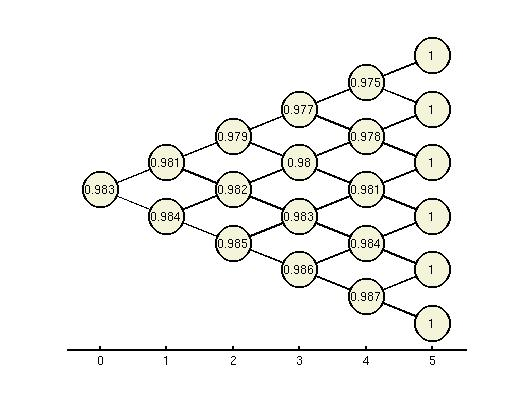
\includegraphics[keepaspectratio=true,scale=0.6]{holeeex1.jpg}}
\captionof{figure}{Ho and Lee zero coupon bond prices where the value in each node is $P_j^n(1)$.}% only if needed
%\label{visina8}
\end{minipage}

\noindent%
\begin{minipage}{\linewidth}
\makebox[\linewidth]{%
  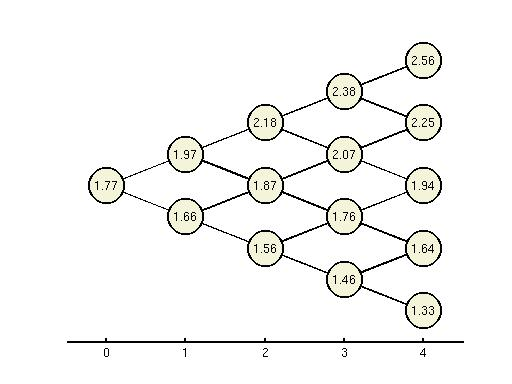
\includegraphics[keepaspectratio=true,scale=0.6]{holeerates.jpg}}
\captionof{figure}{Ho and Lee annually compunded interest rates computed from (1.5.17).}% only if needed
%\label{visina8}
\end{minipage}



%\begin{figure}[H]
%	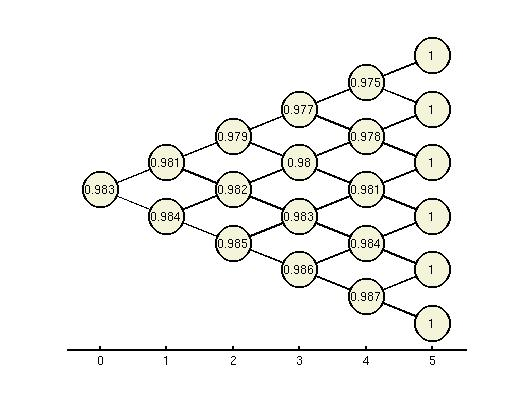
\includegraphics[height=10cm]{holeeex1.jpg}
%	\caption{Ho lee zero coupon bond values}
%\end{figure}	

%\begin{figure}[H]
%	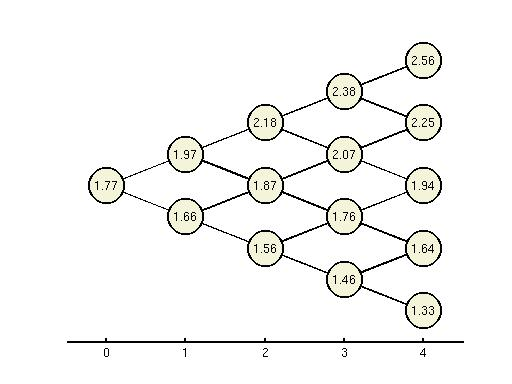
\includegraphics[height=10cm]{holeerates.jpg}
%	\caption{Ho lee interest rates}
%\end{figure}	






%\subsection{The Pedersen, Shiu and Thorlacius Model}
%This model is a generalization of the Ho and Lee model where the risk neutral probabilities are not fixed, but is a function of time.
%\begin{equation}
%\pi(n,j)=\pi(n)\end{equation} for all $j=0,1,2,\cdots,n$ and that
%\begin{equation}
%P_{i+1}^n(1)=P_i^n(1)c(n)\end{equation} for all $i=0,1,2,\cdots,n-1$ given some suitable functions $\pi$ and c . By using
%\begin{equation} P_j^n(T)=P_j^n(1)[\pi(n)P_{j+1}^{n+1}(T-1)+(1-\pi(n))P_j^{n+1}(T-1)] \end{equation} and
%\begin{equation} P_j^n(1)=P_i^n(1)c(n)^{j-i} \,\,for\,\,i,j=0,1,2,\cdots,n. \end{equation} repeatedly we can obtain an equation for $P_j^n(T)$ in terms of one period bond prices. Define
%\begin{equation} g(j,s)=1-\pi(j)+\pi(j)c(j+1)c(j+2)\cdots c(s) \end{equation} for $j<s$, and
%\begin{equation} g(s,s)=1 \end{equation} then $P_j^n(T)$ is given by

%\begin{equation}
%P_j^n(T)=\prod_{k=n}^{T+n-1}g(k,T+n-1)P_j^k(1)\end{equation} applying (1.5.30) twice gives the one period bond prices for each state as

%\begin{equation}
%P_i^n(1)=c(n)^iP_0^n(1)=\frac{P(n+1)}{P(n)}c(n)^i\frac{\prod_{k=0}^{n-2}g(k,n-1)}{\prod_{k=0}^{n-1}g(k,n)}.
%\end{equation}

%By restricting the parameters ${c(1),c(2),\cdots}$ we can ensure that there will be no negative or very high interest rates in the model. Let $M(1),M(2),M(3),\cdots $ be a sequence of numbers all greater than 1. By requiring that $c(n)$ satisfies the inequalities
%\begin{equation} \frac{1}{M(n)}\leq[c(n)]^n\leq M(n) 
%\end{equation} we can ensure that the one period bond prices $P_i^n(1)$ are within the interval
%\begin{equation} \bigg [\frac{P(n+1)}{M(n)P(n)},\frac{M(n)P(n+1)}{P(n)}\bigg ] \end{equation}

%Using (1.5.30) and (1.5.31) we can write $P_i^n(T)$ as
%\begin{equation} P_i^n(T)=\frac{P(T+n)}{P(n)}\bigg [\prod_{k=0}^{n-1}\frac{g(k,n-1)}{g(k,T+n-1)}\bigg ] \bigg [\prod_{j=n}^{T+n-1}c(j^)\bigg ]^i \end{equation} thus the bond price $P_i^n(T)$ does not depend on the risk neutral probabilities \{$\pi(j)|j\geq n$\}.

%We also get
%\begin{equation} P_i^{n+1}(T)=\frac{P_i^n(T+1)}{P_i^n(1)}h(n,T) \end{equation}
%\begin{equation} P_{i+1}^{n+1}(T)=\frac{P_i^n(T+1)}{P_i^n(1)}h^*(n,T) \end{equation}

%where the perturbation functions are given by
%\begin{equation} h(n,T)=\frac{1}{g(n,T+n-1)}\end{equation}
%\begin{equation} h^*(n,T)=c(n+1)c(n+2)\cdots c(T+n-1)g(n,T+n-1) \end{equation}





%Let $R(n,j)\equiv1+r(n,j)$ be the value at time $t=n+1$ of \$1 invested in a bank at time $t=n$ in $(n,j)$ and held until time $t=n+1$. The interest that can be received at time $t=n+1$ starting at time $t=n$ in $(n,j)$ is the quantity $r(n,j)$.

%For a bond choose $T\geq 2$ and define
%\begin{equation}
%\pi(n,j)=\frac{P_j^n(T)\cdot R(n,j)-P_j^{n+1}(T-1)}{P_{j+1}^{n+1}(T-1)-P_j^{n+1}(T-1)}.
%\end{equation} To avoid arbitrage $0\leq \pi(n,j)\leq 1$ for all $(n,j)$.

%A rational price for a contract agreeing to buy a zero-coupon bond with maturity T at time $t=1$ can be show to be
%\begin{equation}
%K=\frac{P(0,T)}{P(0,1)}\end{equation} Thus the 1-forward price of a T-zero when in state $(n,j)$, can be written as
%\begin{equation}
%F_j^n(T)=\frac{P_j^n(T+1)}{P_j^n(1)}
%\end{equation} This motivates the following assumptions
%\begin{assumption}
%There exists functions $h(T)>1>h^*(T)$ so that
%\begin{equation}
%P_{j+1}^{n+1}(T)=\frac{P_j^n(T+1)}{P_j^n(1)}h(T)\end{equation}
%\begin{equation}
%P_j^{n+1}(T)=\frac{P_j^n(T+1)}{P_j^n(1)}h^*(T)\end{equation}
%\begin{equation}
%\pi(n,j)h(T)+(1-\pi(n,j))h^*(T)=1 \end{equation} Also note
%\[\frac{1}{P_j^n(1)}=R(n,j)=1+r(n,j)\]
%\[h(0)=h^*(0)=1\]
%\[\pi(n,j)=\frac{P_j^n(t+1)R(n,j)-P_j^{n+1}(T)}{P_{j+1}^{n+1}(T)-P_j^{n+1}(T)}=\frac{1-h^*(T)}{h(T)-h^*(T)}.\]


%\end{assumption}

%\begin{assumption}
%Bond prices are path independent which implies a recombining tree model. 
%\begin{equation}
%\frac{h(T+1)h^*(T)}{h(1)}=\frac{h^*(T+1)h(T)}{h^*(1)}\end{equation} for all T.
%\end{assumption}

%\begin{assumption}
%$\pi(n,j)=\pi$ is independent of $(n,j)$.
%\end{assumption}

%\begin{lemma}
%\begin{equation}
%h(T)=\frac{1}{\pi+(1-\pi)\delta^T}
%\end{equation}
%\begin{equation}
%h^*(T)=\frac{\delta^T}{\pi+(1-\pi)\delta^T} \end{equation} 
%\end{lemma} Let $P(0,n)$ be written as $P(n)$

%\begin{lemma}
%\begin{equation}
%P_j^n(1)=\frac{P(n+1)}{P(n)}h(n)\delta^{n-j} \end{equation}
%\begin{equation}
%P_j^n(T)=\frac{P(n+T)}{P(n)}\frac{h(T)h(T+1)\cdots h(T+n-1)}{h(0)h(1)\cdots h(n-1)}\delta^{(n-j)T} \end{equation}
%\end{lemma} The Ho and Lee model will sometimes have problems with negative interest rates (r(n,j)), so that $\pi$ and $\delta$ must be carefully chosen in order to prevent this from happening.



%Assets who depend on interest rates are called fixed income assets. The simplest fixed income asset is a zero-coupon bond, a bond that pays a specified amount called \textsl{face value} at a specified time (maturity). At times prior to maturity the value of this asset is less than its face value, provided that the interest rate is always greater than zero.

%The \textsl{yield} of the zero-coupon bond corresponding to a given maturity is defined as the constant interest rate that would be needed so that the time-zero price of the bond invested at time zero and allowed to accumulate at this interest rate would grow to the face value of the bond at the bond's maturity. The \textsl{yield curve} is the function from the maturity variable to the yield variable. 

%Term structure of interest rate models provide a method for random evolution of the yield curve forward in time. By building the model under the risk-neutral measure we avoid the problem of arbitrage. We first describe the evolution of the interest rate under the risk-neutral measure, then determine the prices of zero coupon bonds and all other fixed income assets by using the risk-neutral pricing formula.

%\newline % new line
%Let $P(t,T)$ be the value at time t of a zero-coupon bond expiring at time T with face value of 1 in a given currency. Interest modelling can be specified by modelling various variables using short term or forward rates.

%\begin{itemize}
%\item[1.] $P(t,T)$.
%\item[2.] $y(t,T)$ the yield to maturity defined through
%\[P(t,T)=\exp{(-y(t,T)\cdot(T-t))}\]
%\[y(t,T)=-\frac{1}{T-t}\ln P(t,T).\]
%\item[3.] $r(t)\equiv f(t,t)$ the spot rate and
%\[P(t,T)=\mathbb E\Bigg[exp(-\int_t^Tr(u)\,du)\mid \mathbb F_t \Bigg].\] where $\mathbb F_t\equiv\sigma\{r(u)\mid0\leq u\leq t\}$ represents the past history on the spot rates up to the time t.
%\item[4.] $f(t,T)$ the forward rate defined in continuous time through
%\[P(t,T)=exp\Bigg(-\int_t^Tf(t,u)\,du\Bigg)\]
%\[f(t,T)=-\frac{\partial}{\partial T}\ln P(t,T).\]


%\end{itemize} %We want to be able to determine values for $R(n,j) = 1 + r(n,j)$ and $\pi(n,j)$ for the nodes in our tree models. This %will enable us to price contingent claims and thus we can also compute $P(t,T)$ for various values of $(t,T)$.





%\section{Binomial Model for Interest Rates}\label{Binomial}

%Let $\Omega$ be the set of $2^N$ possible outcomes $\omega_{1}\omega_{2}\cdots\omega_N$ of N tosses of a coin, and let $\mathbb P$ be a probability measure on $\Omega$ under which every sequence $\omega_1\omega_2\cdots\omega_N$ has strictly positive probability.

%An interest rate process is defined to be a sequence of random variables $R_0,R_1,\cdots,R_{N-1}$, where $R_0$ is not random, and for n=1,...,N-1, $R_n$ depends only on the first n coin tosses $\omega_1\cdots\omega_n$. 

%Since we at time n know the interest rate what will be applied to money market investments for the period from time n to the time n+1, one dollar invested in the money market will grow to $1+R_n$ dollars during that time period. Although $R_n$ is assumed to be greater than zero for all n and all $\omega_1\cdots\omega_n$, the analysis only requires that
%\begin{equation}R_n(\omega_1\cdots\omega_n) > -1 \end{equation}  for all n and all $\omega_1\cdots\omega_n$. The discount process can then be defined by
%\begin{equation}D_n = \frac{1}{(1+R_0)\cdots(1+R_{n-1})} , n=1,2,\cdots,N;\, D_0=1 \end{equation}


%By the risk-neutral pricing formula the value at time zero if a payment X received at time m is $\mathbb E[D_mX]$. Using this formula we can define the time zero price of a zero-coupon bond that pays 1 at maturity time m to be
%\begin{equation}B_{0,m}=\mathbb E[D_m].\end{equation} The yield for this bond is the number $y_m$ for which
%\begin{equation}\frac{1}{B_{0,m}}=(1+y_m)^m.\end{equation} This equation can then be solved for $y_m$:
%\begin{equation}y_m=(\frac{1}{B_{0,m}})^\frac{1}{m}-1 \end{equation}

%\begin{definition} Let $\mathbb P$ be a probability measure on the space $\Omega$ of all possible sequences of N coin tosses. Assume that every sequence $\omega_1\cdots\omega_N$ in $\Omega$ has positive probability under $\mathbb P$. Let $1\leq{n}\leq{N-1}$, and let $\bar{\omega}_1\cdots\bar{\omega}_N$ be a sequence of N coin tosses. We define
%\begin{multline}\mathbb P\{\omega_{n+1}=\bar\omega_{n+1},\cdots,\omega_N=\bar\omega_N|\omega_1=\bar\omega_1,\cdots,\omega_n=\bar\omega_n\} \\ =\frac{\mathbb P\{\bar\omega_1\cdots\bar\omega_n\bar\omega_{n+1}\cdots\bar\omega_N\}}{\mathbb P\{\omega_1=\bar\omega_1,\cdots,\omega_n=\bar\omega_n\}}
%\end{multline} Let X be a random variable. We define the conditional expectation of X based on the information at time n by the formula
%\begin{multline}\mathbb E_n[X](\bar\omega_1\cdots\bar\omega_n)=\sum_{\bar\omega_{n+1},\cdots,\bar\omega_N}X(\bar\omega_1\cdots\bar\omega_n\bar\omega_{n+1}\cdots\bar\omega_N) \\
%\times\mathbb P\{\omega_{n+1}=\bar\omega_{n+1},\cdots,\omega_N=\bar\omega_N|\omega_1=\bar\omega_1,\cdots,\omega_n=\bar\omega_n\}.
%\end{multline}
%\end{definition}

%\begin{definition} (Zero-coupon bond prices) Let $\mathbb P$ be a probability measure on the space $\Omega$ of all possible sequences of N coin tosses, and assume that every sequence $\omega_1\cdots\omega_N$ has strictly positive probability under $\mathbb P$. Let $R_0,R_1,\cdots,R_{N-1}$ be an interest rate process, with each $R_n$ depending on only the first n coin tosses and satisfying (1.2.1). Define the discount process $D_n,$ $n=0,1,\cdots,N$ by (1.2.2). For $0\leq n\leq m\leq N$, the price at time n of the zero-coupon bond maturing at time m is defined to be
%\begin{equation}B_{n,m}=\mathbb E[\frac{D_m}{D_n}]\end{equation}
%\end{definition}

%If we consider an agent that can trade in zero-coupon bonds of every maturity and in the money arket, we can show that the wealth of such an individual, when discounted, constitutes a martingale. Thus the model where the zero-coupon bond prices we defined by (1.2.4) will have no arbitrage opportunities. The agent begins with an initial wealth of $X_0$ and have a wealth of $X_n$ at time n. Let $\Delta_{n,m}$ be the number of m maturity zero-coupon bonds held between times n and n+1. The agents wealth at time n+1 is given by
%\begin{equation}X_{n+1}=\Delta_{n,n+1}+\sum_{m=n+2}^N\Delta_{n,m}B_{n+1,m}+(1+R_n)(X_n-\sum_{m=n+1}^N\Delta_{n,m}B_{n,m})\end{equation}

%\begin{theorem} Regardless of how the portfolio random variables $\Delta_{n,m}$ are chosen subject to the condition that $\Delta_{n,m}$ may only depend on the first n coin tosses), the discounted wealth process $D_nX_n$ is a martingale under $\mathbb P$.
%\end{theorem}

%Let $0\leq m\leq N$ be given. A \textsl{coupon paying bond} can be modeled as a sequence of constant quantities $C_0,C_1,\cdots,C_m$. For $0\leq n\leq m-1$, the constant $C_n$ is the coupon payment made at time n. The constant $C_m$ is the payment made at time m, which includes principal as well as any coupon due at time m. A coupon paying bond can be regarded as a sum of $C_1$ zero-coupon bonds maturing at time 1, $C_2$ zero-coupon bonds maturing at time 2, etc. up to $C_m$ zero-coupon bonds maturing at time m. The price at time zero of the coupon paying bond is thus
%\begin{equation}\sum_{k=0}^mC_kB_{0,k}=\mathbb E[\sum_{k=0}^mD_kC_k]\end{equation} At time n, before the payment $C_n$ has been made, but after the payments $C_0,C_1,\cdots,C_{n-1}$ have been made, the price of the coupon paying bond is
%\begin{equation}\sum_{k=n}^mC_kB_{n,k}=\mathbb E_n\Bigg[\sum_{k=n}^m\frac{D_kC_k}{D_n}\Bigg], n=0,\cdots,m.\end{equation}

%%%%%%%%%
% Inserts specific short rate models.
%\section{Short Rate Interest Models}
%\subsection{P(0,T) from Treasury Data}

%Let us assume that a bond that expires at $T_n$ has coupon payments of C at $T_1,T_2,\cdots,T_n$. It has a present value
%\begin{equation}
%P=\sum_{i=1}^nC\,P(0,T_i)+F\,P(0,T_n)\end{equation} where F is the face value of the bond and C is a given percentage of F.

%\subsection{P(0,T) from Bank Data}

%\textbf{Swap Rates}

%Let $r_t$ be the variable rate known at t that applies between times t and $t+\delta$. Since 1 dollar invested at t grows to $1+r_t\delta$ at time $t+\delta$
%\begin{equation}
%(1+r_t\delta)P(t,t+\delta)=1
%\end{equation}
%it follows that
%\begin{equation}
%r_t\equiv r_{t,t+\delta}=\frac{1}{\delta}\Bigg[\frac{1}{P(t,t+\delta)}-1\Bigg].
%\end{equation}
%Assume a swap is performed at time $t+\delta$. A payer-swap is one in which a fixed rate is paid and a floating rate is received. A receiver-swap has the reverse cash flow. Let F be the face value and $\kappa$ be the fixed rate, the net flow can be written as
%\begin{equation}
%F\cdot r_t\cdot\delta-F\cdot\kappa\cdot\delta
%\end{equation}
%The present value (at time 0) is then
%\begin{equation}
%PV=F\cdot P(0,t)-F\cdot(1+\kappa\delta)\cdot P(0,t+\delta)
	%=F\cdot[P(0,t)-P(0,t+\delta)]-F\cdot\kappa\cdot\delta\cdot P(0,t+\delta).
%\end{equation}

%The present value of the cash flows from a payer-swap where interest is exchanged at times $\delta,2\delta,\cdots,n\delta$ is
%\begin{equation}
%PV=F\cdot [1-P(0,n\delta)]-F\cdot\kappa\cdot\delta\cdot[P(0,\delta)+P(0,2\delta)+\cdots+P(0,n\delta)]
%\end{equation}
%Setting PV=0 and solving for the swap rate $\kappa$ we get
%\begin{equation}
%\kappa=\frac{1}{\delta}\Bigg[\frac{1-P(0,n\delta)}{P(0,\delta)+P(0,2\delta)+\cdots+P(0,n\delta)}\Bigg].
%\end{equation}

%Let $\delta=0.5$, for semiannual swaps, and $\delta=0.25$ for quarterly swaps. $\kappa(nQ)$ is the n-year quarterly swap rate, and $\kappa(nS)$ the n-year semiannual swap rate.

%\subsection{Computing $P(0,t)$ from Market Data}
%In the AA market bank bill swap rates (BBSW) are provided for 30, 60, 90, 120, 150 and 180 days. Then P(0,t) can be given by a %discounting formula. For example 
%\begin{equation}
%P(0,0.25)=P(0,\frac{3}{12})=\frac{1}{1+\frac{90}{360}\cdot i_{90}}
%\end{equation}
%where $i_{90}$ is the 90 day BBSW interest rate. The AA arket also provides 1Q, 2Q, 3Q (quarterly swap rates) and 4S, 5S, 7S, 10S, 15S and 20S (semiannual) swap rates. The approximation
%\begin{equation}
%\kappa(nS)=2\Bigg[\Bigg[1+\frac{\kappa(nQ)}{4}\Bigg]^2-1\Bigg] \end{equation} are often used when quarterly swap data are given (1Q,2Q,3Q).

%finish this later and repeat.


%\subsection{Computing P(0,T) from Market Data - A Second Version}
%Another version that is used is to set
%\begin{equation}
%\kappa((n+0.5)S)=0.5(\kappa(nS)+\kappa((n+1)S).
%\end{equation} Once these values are known we can calculate $P(0,n+0.5)$ in terms of $P(0,n)$ whenever n is a multiple of 0.5.
%\begin{equation}
%\kappa((n+0.5)S)=2\Bigg[\frac{1-P(0,n+0.5)}{\frac{2(1-P(0,n))}{\kappa(nS)}+P(0,n+0.5)}\Bigg].
%\end{equation} Which can be rearranged to give
%\begin{equation}
%P(0,n+0.5)=\Bigg[1+\frac{\kappa((n+0.5)S)}{2}\Bigg]^{-1}\Bigg[1-\frac{\kappa((n+0.5)S)}{\kappa(nS)}(1-P(0,n))\Bigg]
%\end{equation}

%\subsection{Interpolation of P(0,T)}
%If we know $P(0,T_1)$ and $P(0,T_2)$ we can estimate $P(0,T)$ where $T_1\leq T\leq T_2$ by
%\begin{equation}
%P(0,T)=P(0,T_1)^{1-\alpha}P(0,T_2)^\alpha\end{equation}
%where
%\begin{equation}
%\alpha=\frac{T-T_1}{T_2-T_1}
%\end{equation} These interpolated values of $P(0,t)$ can be used to discount cash flows that fall on dates that are not integer multiples of 0.5 years ahead.

%\subsection{Other Discount Curves}
%We can now compute $\tilde{P}(0,t)$ for less creditworthy entities. We then have $\tilde{P}(0,t)<P(0,t)$ for each t, but still $\tilde{P}(0,0)=P(0,0)=1$. If we are considering the AA curve $\tilde{P}(0,t)>P(0,t)$, if P(0,t) stands for AA values and $\tilde{P}(0,t)$ is a goverment bond (higher credit rating). Lets consider a bond that pays a coupon semi-annually at $c_1$\% per annum (that is it pays $\frac{F\cdot(c_1/100))}{2}$ every six months. If the yield to maturity $y_1$\% is quoted, the value of this bond is be given by
%\begin{equation}
%MS1=\frac{c_1}{2}\Bigg[\frac{1}{(1+\frac{y_1}{2})}+\frac{1}{(1+\frac{y_1}{2})^2}+\cdots+\frac{1}{(1+\frac{y_1}{2})^{m_1}}\Bigg]+\frac{1}{(1+\frac{y_1}{2})^{m_1}}
%\end{equation} where $m_1$ is the number of coupons paid. This equation can be simplified to
%\begin{equation}
%MS1=\frac{c_1}{y_1}\Bigg[1-(1+\frac{y_1}{2})^{-m_1}\Bigg]+(1+\frac{y_1}{2})^{-m_1}.
%\end{equation} Once a value of $\tilde{P}(0,t)$ has been computed, the adjusted swap rates can be calculated from
%\begin{equation}
%\tilde{\kappa}((n+0.5)S)=2\Bigg[\frac{1-\tilde{P}(0.n+0.5)}{\frac{2(1-\tilde{P}(0.n))}{\tilde{\kappa}(nS)}+\tilde{P}(0,n+0.5)}\Bigg]
%\end{equation} for $n=0,0.5,1,1.5,\cdots$ using  $\tilde{P}(0,0)=1$.


%\subsection{The Ho and Lee model}
%Let each node in a binomial tree have a label $(n,j)$. The label n refers to time $n=0,1,2,\cdots$, and j numbers the states $j=0,1,2,\cdots,n$. Thus there are n+1 states at time n. If we at time 0 are in node $(0,0)$, then at time n=1 we are in either node $(1,1)$ or $(1,0)$. Thus we either move up or down from the starting node. 

%Define $P_j^{(n)}(T)$ to be the value at time $t=n$ in state j of \$1 at time $t=T+n$ (T periods after t=n). Let $R(n,j)\equiv1+r(n,j)$ be the value at time $t=n+1$ of \$1 invested in a bank at time $t=n$ in $(n,j)$ and held until time $t=n+1$. The interest that can be received at time $t=n+1$ starting at time $t=n$ in $(n,j)$ is the quantity $r(n,j)$.

%For a bond choose $T\geq 2$ and define
%\begin{equation}
%\pi(n,j)=\frac{P_j^n(T)\cdot R(n,j)-P_j^{n+1}(T-1)}{P_{j+1}^{n+1}(T-1)-P_j^{n+1}(T-1)}.
%\end{equation} To avoid arbitrage $0\leq \pi(n,j)\leq 1$ for all $(n,j)$.

%A rational price for a contract agreeing to buy a zero-coupon bond with maturity T at time $t=1$ can be show to be
%\begin{equation}
%K=\frac{P(0,T)}{P(0,1)}\end{equation} Thus the 1-forward price of a T-zero when in state $(n,j)$, can be written as
%\begin{equation}
%F_j^n(T)=\frac{P_j^n(T+1)}{P_j^n(1)}
%\end{equation} This motivates the following assumptions
%\begin{assumption}
%There exists functions $h(T)>1>h^*(T)$ so that
%\begin{equation}
%P_{j+1}^{n+1}(T)=\frac{P_j^n(T+1)}{P_j^n(1)}h(T)\end{equation}
%\begin{equation}
%P_j^{n+1}(T)=\frac{P_j^n(T+1)}{P_j^n(1)}h^*(T)\end{equation}
%\begin{equation}
%\pi(n,j)h(T)+(1-\pi(n,j))h^*(T)=1 \end{equation} Also note
%\[\frac{1}{P_j^n(1)}=R(n,j)=1+r(n,j)\]
%\[h(0)=h^*(0)=1\]
%\[\pi(n,j)=\frac{P_j^n(t+1)R(n,j)-P_j^{n+1}(T)}{P_{j+1}^{n+1}(T)-P_j^{n+1}(T)}=\frac{1-h^*(T)}{h(T)-h^*(T)}.\]


%\end{assumption}

%\begin{assumption}
%Bond prices are path independent which implies a recombining tree model. 
%\begin{equation}
%\frac{h(T+1)h^*(T)}{h(1)}=\frac{h^*(T+1)h(T)}{h^*(1)}\end{equation} for all T.
%\end{assumption}

%\begin{assumption}
%$\pi(n,j)=\pi$ is independent of $(n,j)$.
%\end{assumption}

%\begin{lemma}
%\begin{equation}
%h(T)=\frac{1}{\pi+(1-\pi)\delta^T}
%\end{equation}
%\begin{equation}
%h^*(T)=\frac{\delta^T}{\pi+(1-\pi)\delta^T} \end{equation} 
%\end{lemma} Let $P(0,n)$ be written as $P(n)$

%\begin{lemma}
%\begin{equation}
%P_j^n(1)=\frac{P(n+1)}{P(n)}h(n)\delta^{n-j} \end{equation}
%\begin{equation}
%P_j^n(T)=\frac{P(n+T)}{P(n)}\frac{h(T)h(T+1)\cdots h(T+n-1)}{h(0)h(1)\cdots h(n-1)}\delta^{(n-j)T} \end{equation}
%\end{lemma} The Ho and Lee model will sometimes have problems with negative interest rates (r(n,j)), so that $\pi$ and $\delta$ must be carefully chosen in order to prevent this from happening.

%\subsection{The Pedersen, Shiu and Thorlacius Model}
%This model is a generalization of the Ho and Lee model. Instead of Assumption 3, they assume that
%\begin{equation}
%\pi(n,j)=\pi(n)\end{equation} for all $j=0,1,2,\cdots,n$ and that
%\begin{equation}
%P_{i+1}^n(1)=P_i^n(1)c(n)\end{equation} for all $i=0,1,2,\cdots,n-1$, for suitable functions $\pi$ and c. It can be show that
%\begin{equation}
%P_j^n(T)=\prod_{k=n}^{T+n-1}g(k,T+n-1)P_j^k(1)\end{equation} where
%\[g(j,s)=1-\pi(j)+\pi(j)c(j+1)c(j+2)\cdots c(s) \] for $j<s$, and
%\[g(s,s)=1\] and
%\begin{equation}
%P_i^n(1)=c(n)^iP_0^n(1)=\frac{P(n+1)}{P(n)}c(n)^i\frac{\prod_{k=0}^{n-2}g(k,n-1)}{\prod_{k=0}^{n-1}g(k,n)}.\end{equation}

%\subsection{The Morgan and Neave Model}
%This model has one parameter $u>1$. For $n=0,1,2,\cdots$ set
%\begin{equation}
%R(n)=\frac{P(n)}{P(n+1)}\equiv\frac{P(0,n)}{P(0,n+1)}>1\end{equation} and define for $j=0,1,2,\cdots,n$
%\begin{equation}
%R(n,j)=R(n)u^{n-2j}.\end{equation} The model assume that $\pi(n,j)=\pi(n)$ are independent of j. This forces
%\begin{equation}
%\pi(n)=\frac{1}{1+u^{2n+1}}\end{equation} to hold for all n, and
%\begin{equation}
%P_{j+1}^n(T)=u^{2T}P_j^n(T)\end{equation} for all $(n,j)$ and T. It can be further shown that
%\begin{equation}
%P_j^n(T)=u^{2Tj}\prod_{k=n}^{T+n-1}\Bigg[\frac{\pi(k)u^{2(T+n-1-k)}+(1-\pi(k))}{u^kR(k)}\Bigg]\end{equation}




%\subsection{The Black, Derman and Toy Model}
%In this model it is assumed that
%\begin{equation}
%\pi(n,j)\equiv\frac{1}{2}\end{equation}
%\begin{equation}
%r(n,j)=r(n,0)\sigma(n)^j\end{equation} where $\sigma(n)$ for $n=1,2,\cdots$, are specified constants. This model can be calibrated to be consistent with observed values of $P(0,n)$ for various n, and that interest rates $r(n,j)$ are all positive.



%\subsection{Defaultable Bonds}
%Let $V(n,j)$ be the value of a corporation at time $t=n$ in state j. At $t=0$ it is funded from equity S(0,0) and debt B(0,0) as
%\begin{equation}
%V(0,0)=S(0,0)+B(0,0)\end{equation}
%At time N the debt becomes due and must be repaid by the firm. The debt holders will receive
%\begin{equation}
%\tilde{B}(N,j)=min[V(N,j),B]\end{equation} at time N. The the present value of $\tilde{B}(N,\cdot)$ is
%\begin{equation}
%B(0,0)=B\tilde{P}(0,N)\end{equation} If it is possible that $V(N,j)<B$ in some state j, it can be shown that $\tilde{P}(0,N)<P(0,N)$. This enables us to find the value of defaultable zero-coupon bonds given a binomial tree with values \{${V(n,j),\pi(n,j)}$\}. 

\chapter{Forward Interest Rate Modeling}

\section{Forward Interest Rates}

The references used are [1],[8]. Let $t\leq T\leq S$. There will often be a need to agree at present time t for a loan for some future time period $[T,S]$. The interest rate applied to this loan is called a forward rate and is denoted by $f(t,T,S)$.

\begin{definition} The continuously compounded forward rate f(t,T,S) at time t for a loan on $[T,S]$ is given by
\begin{equation} f(t,T,S)=-\frac{ln \,P(T,S)-ln\, P(t,T)}{S-T} \end{equation} where the continuously compounded spot forward rate F(t,T) is given by
\begin{equation} F(t,T) := f(t,t,T)=-\frac{ln \,P(t,T)}{T-t} \end{equation} which is identical to the continuously compounded spot rate R(t,T).
\end{definition} By taking the limit of the forward rate $f(t,T,S)$ as $S\rightarrow T^+$ we get the instantaneous forward rate $f(t,T)$
\begin{equation} f(t,T):= - \underset{S\rightarrow T^+}{lim} \frac{ln \,P(t,S)-ln \,P(t,T)}{S-T}=-\frac{\partial ln\,P(t,T)}{\partial T}=-\frac{1}{P(t,T)}\frac{\partial P(t,T)}{\partial T}. \end{equation} Solving this as a differential equation using the initial condition $P(T,T)=1$ gives

\begin{equation} ln \,P(t,T)=ln \,P(t,T)-ln \,P(t,t)=\int_t^T\frac{\partial ln \,P(t,s)}{\partial s}ds=-\int_t^Tf(t,s)\, ds \end{equation}
\begin{equation} P(t,T)= exp \bigg (-\int_t^Tf(t,s) \, ds \bigg )\,\,\,\,0\leq t\leq T \end{equation} The forward rate $f(t,T,S)$ can be recovered from the instantaneous forward rate
\begin{equation} f(t,T,S)= \frac{1}{S-T}\int_T^S f(t,s)\,\,ds\,\,\,0\leq t\leq T<S \end{equation} When the short rate $(r_t)_{t\in \mathbb R^+}$ is a deterministic function we have
\begin{equation} P(t,T)=exp \bigg (-\int_t^Tf(t,s)ds \bigg )=exp \bigg (-\int_t^T r_s ds\bigg ) \end{equation} The relationship of the forward rate and the short rate can be seen as follows
\begin{equation} P(t,T)= E \bigg[exp \bigg (-\int_t^T r_sds\bigg ) | r_t \bigg] \end{equation} so we have

\[ \frac{\partial P}{\partial T}(t,T)=\frac{\partial}{\partial T} E \bigg[exp \bigg( -\int_t^Tr_s ds \bigg) |r_t \bigg] \]
\[ =E\bigg [ \frac{\partial}{\partial T} exp \bigg( -\int_t^Tr_s ds \bigg) |r_t \bigg] \]
\[ =E \bigg[r_T \,exp\bigg (-\int_t^Tr_s ds \bigg )|r_t \bigg]. \] it follows that the limit

\begin{equation}
\underset{T\rightarrow t^+}{lim} \frac{\partial P}{\partial T}(t,T)=-  E[r_t|r_t]=-r_t
\end{equation} the limit as $T\rightarrow t^+$ of instantanous forward rate equals the short rate $r_t$
\begin{equation} \underset{T\rightarrow t^+}{lim} f(t,T)=- \underset{T\rightarrow t^+}{lim} \frac{1}{P(t,T)}\frac{\partial P(t,T)}{\partial T}=r_t \end{equation}



\section{Fixed-Income Derivatives}

The reference used for chapters 2.2-2.4 is [9]. A derivative security is a security whose payoff depends on one or more underlying securities or variables. A well known example of a derivative security is a call option on a stock, which gives the buyer of the call the right to buy the stock on a specific date at a specified price. We consider a binomial model over a time period $[0,\tau]$, where the dates $n,m$ are specified as $0\leq n\leq m\leq \tau$. Let $S_n$ be the price of an asset at time $n$. If the price $S_n$ depends on the first $n$ coin tosses, then the discounted asset price will be a martingale under the risk neutral measure $Q$.
\begin{equation}D(0,n)S_n= E^Q[D(0,n+1)S_{n+1}|\mathcal{F}_n], \,\,n=0,1,\cdots,\tau-1\end{equation}

\begin{definition} A forward contract is an agrement to pay a delivery price $K$ at a delivery date $m$ for the asset whose price at time $m$ is $S_m$. The $m$-forward price of this asset at time $n$ is the value of $K$ that makes the forward contract have no arbitrage price zero at time $n$. \end{definition} If we consider an asset whose price process is $S_0,S_1,\cdots,S_\tau$ in the binomial model, then the $m$-forward price at time $n$ is
\begin{equation} For(n,m)=\frac{S_n}{P(n,m)} \end{equation} For the time period $0\leq n\leq m\leq \tau-1$, the annually compounded forward interest rate can be defined as
\begin{equation} F_r(n,m)=\frac{P(n,m)}{P(n,m+1)}-1=\frac{P(n,m)-P(n,m+1)}{P(n,m+1)} \end{equation} which is the forward interest rate at time $n$ for investing at time $m$.

\subsection{Swaps}
An interest rate swap is an agreement between two parties who each make a contract to pay the other on some specified dates in the future. One agent receives constant payments at each time, while the other receives a variable amount whose size depend on the future rates of interest. Thus an agent can use swaps to convert a fixed interest rate loan into a variable interest rate loan or vice versa.

Let $1\leq m\leq \tau$. An $m$-period interest rate swap is a contract that pays $S_1,\cdots,S_m$ at times $1,\cdots,m$ where
\begin{equation} S_n=K-r(n-1), \,\,\,n=1,\cdots,m \end{equation} where $r(n-1)$ is the annually compounding rate. The fixed rate $K$ is constant. The value of $K$ that makes the time zero no arbitrage price of the interest rate swap equal to zero is denoted $SR_m$. The time zero no arbitrage price of the $m$-period interest rate swap is
\begin{equation} Swap_m=\sum_{n=1}^mP(0,n)(K-F_r(0,n-1)=K\sum_{n=1}^m P(0,n)-(1-P(0,m)) \end{equation}
\begin{equation} SR_m=\frac{\sum_{n=1}^m P(0,n)F_r(0,n-1)}{\sum_{n=1}^m P(0,n)} = \frac{1-P(0,m)}{\sum_{n=1}^m P(0,n)} \end{equation} In the binomial model it can be shown that the risk neutral price of the swap is
\begin{equation} Swap_m=E^Q \bigg [\sum_{n=1}^mD(0,n)(K-r(n-1)) \bigg] \end{equation}

\subsection{Caps and Floors}

Caps and Floors are usually bought to insure against rises and falls in the money market interest rates. Let $1\leq m\leq \tau$. An $m$-period interest rate cap is a contract that pays $C_1,\cdots,C_m$ at times $1,\cdots,m$ where 
\begin{equation} C_n=(r(n-1)-K)^+ \end{equation} An interest rate floor is a contract that makes payments $F_1,\cdots,F_m$ at times $1,\cdots,m$ where
\begin{equation} F_n=(K-r(n-1))^+ \end{equation} If the contract only makes a single payment at time $n$ it is called a caplet or floorlet respectively. Thus a cap or floor contract will pay the difference if the interest rates raises above or falls below a certain level. The risk neutral price of an $m$-period cap is
\begin{equation} Cap_m=E^Q\bigg [\sum_{n=1}^m D(0,n)(r(n-1)-K)^+\bigg ] \end{equation} and the risk neutral price of an m-period interest rate floor is \begin{equation} Floor_m=E^Q\bigg [\sum_{n=1}^m D(0,n)(K-r(n-1))^+\bigg ] \end{equation}

\section{Forward Measures}

Denote the payoff at time $m$ of some contract as $V_m$. The risk neutral price of this security at time $n$ is
\begin{equation} V_n=\frac{1}{D(0,n)}E^Q[D_mV_m|\mathcal{F}_n] \end{equation} It is difficult to compute the conditional expectation when $D_m$ is random as one would have to know the joint conditional distribution of $D_m$ and $V_m$ under the risk neutral measure. By using $D_m$ as a Radon-Nikodym derivative one can change the probability measure from a risk neutral measure to a forward measure. Since the term $D_m$ no longer appears in the formula we can then compute expectations more easily using the new measure.

\begin{definition} In a $\tau$ period binomial model let $P$ be the actual probability measure and $Q$ the risk neutral probability measure. Assume that P($\omega$)>0 and Q($\omega$)>0 for all $\omega$. Let $Z(\omega)=\frac{Q(\omega)}{P(\omega)}$ (state price density) for every $\omega$. The Radon-Nikodym derivative process is
\begin{equation} Z_n=E[Z|\mathcal{F}_n],\,\,\,n=0,1,\cdots,\tau \end{equation} Note that $Z_\tau$=Z and $Z_0$=1. \end{definition}
\begin{definition} Let $1\leq m \leq \tau$. Define
\begin{equation} Z_{m,m}=\frac{D(0,m)}{P(0,m)} \end{equation} the $m$-forward measure $P^m$ is defined by
\[P^m(\omega)=Z_{m,m}(\omega)Q(\omega)\,\,for\,all\,\omega\in\Omega \] \end{definition} \noindent We may then define the Radon-Nikodym derivative process as
\begin{equation} Z_{n,m}=E^Q[Z_{m,m}|\mathcal{F}_n]\,\,n=0,1,\cdots,m \end{equation} If $V_m$ is a random variable only depending on the first $m$ coin tosses then
\begin{equation} E^m[V_m]=E^Q[Z_{m,m}V_m] \end{equation} Also if $0\leq n\leq m$
\begin{equation} E^m[V_m|\mathcal{F}_n]=\frac{1}{Z_{n,m}}E^Q[Z_{m,m}V_m|\mathcal{F}_n] \end{equation} this can be rewritten as
\begin{equation} Z_{n,m}=\frac{D(0,n)P(n,m)}{P(0,m)} \end{equation}
\begin{theorem} Let $1\leq m\leq \tau$, and let $P^m$ denote the $m$-forward measure. If $V_m$ is a random variable depending only on the first $m$ coin tosses then
\begin{equation} E^m[V_m]=\frac{1}{P(0,m)} E^Q[D_mV_m] \end{equation} in general
\begin{equation} E^m[V_m|	\mathcal{F}_n]=\frac{1}{D(0,n)P(n,m)} E^Q[D(0,m)V_m|\mathcal{F}_n] \end{equation}
\end{theorem}

\section{Futures}

A shortcoming of forward contracts is that on any date prior to the delivery date there can be a demand for forward contracts with that delivery date. For the market to be efficient there would have to be a supply of forward contracts with different initiation dates for each delivery date. A futures contract is a contract that locks in the price of an asset before the time of purchase or sale. Thus the futures price is tied to a delivery date, but not an initiation date.
\begin{definition} Assume we are considering an asset with price process   \,\, \,$S_0$,$S_1$,$\cdots$,$S_\tau$ in the binomial model. For $0\leq m\leq \tau$, the $m$-futures price process $Fut_{n,m}$, where $n=0,1,\cdots,m$ is an adapted process with the following properties
\begin{itemize}
\item[a)] $Fut_{m,m}=S_m$ 
\item[b)] For each $n$, $0\leq n\leq m-1$ the risk neutral value at time $n$ of the contract that receives the payments $Fut_{k+1,m}-Fut_{k,m}$ at time $k+1$ for all $k=n,\cdots,m-1$ is zero
\begin{equation} \frac{1}{D(0,n)}E^Q\bigg [\sum_{k=n}^{m-1}D(0,k+1)(Fut_{k+1,m}-Fut_{k,m}) |\mathcal{F}_n \bigg] =\,0 \end{equation}
\end{itemize} \end{definition}

The unique process that satisifies the conditions in definition (2.4.1) is
\begin{equation} Fut_{n,m}=E^Q[S_m	|\mathcal{F}_n],\,\,n=0,1,\cdots,m \end{equation}

%Let $S_n$ be the price at time n for a given asset. If the price $S_n$ is dependent on the first n coin tosses, the discounted asset price under $\mathbb P$ is a martingale;

%\begin{equation}D_nS_n=\mathbb E_n[D_{n+1}S_{n+1}], \,n=0,1,\cdots,N-1\end{equation}

%\begin{definition}
%A forward contract is an agreement to pay a specified delivery price K at a delivery date m, where $0\leq m\leq N$, for the asset whose price at time m is $S_m$. The m-forward price of this asset at time n, where $0\leq n\leq m$, is the value of K that makes the forward contract have no-arbitrage price zero at time n.
%\end{definition}

%\begin{theorem}
%Consider an asset with price process $S_0,S_1,\cdots,S_N$ in the binomial interest rate model. Assume that zero-coupon bonds of all maturities can be traded. For $0\leq n\leq m\leq N$, the m-forward price at time n of the asset is

%\begin{equation}For_{n,m}=\frac{S_n}{B_{n,m}}.\end{equation}
%\end{theorem}

%\begin{definition}
%Let $0\leq n\leq m\leq N-1$ be given. The forward interest rate at time n for investing at time m is defined by
%\begin{equation}F_{n,m}=\frac{B_{n,m}}{B_{n,m+1}}-1 = \frac{B_{n,m}-B_{n,m+1}}{B_{n,m+1}} \end{equation} Also note that $F_{m,m}=R_m$.
%\end{definition}

%\begin{theorem} Let $0\leq n\leq m\leq N-1$ be given. The no-arbitrage price at time n of a contract that pays $R_m$ at time m+1 is $B_{n,m+1}F_{n,m}=B_{n,m}-B_{n,m+1}$.
%\end{theorem}

%\begin{definition} Let m be given with $1\leq m\leq N$. An m-period interest rate swap is a contract that make payments $S_1,\cdots,S_m$ at times $1,\cdots,m$, respectively, where
%\begin{equation}S_n=K-R_{n-1},\,n=1,\cdots,m.\end{equation} The fixed rate K is constant. The m-period swap rate $SR_m$ is the value of K that makes the time-zero no-arbitrage price of the interest rate swap equal to zero.
%\end{definition}

%\begin{theorem}
%fiks peker til rett definisjon
%The time-zero no-arbitrage price of the m-period interest rate swap in Definition (1.3.5) is
%\begin{equation}Swap_m=\sum_{n=1}^mB_{0,n}(K-F_{0,n-1})=K\sum_{n=1}^mB_{0,n}-(1-B_{0,m}).\end{equation} In particular, the m-period swap rate is
%\begin{equation}SR_m=\frac{\sum_{n=1}^mB_{0,n}F_{0,n-1}}{\sum_{n=1}^mB_{0,n}}=\frac{1-B_{0,m}}{\sum_{n=1}^mB_{0,n}}.\end{equation}
%\end{theorem} It can be shown that the risk-neutral price of the swap is
%\begin{equation}Swap_m=\mathbb E\sum_{n=1}^mD_n(K-R_{n-1}).\end{equation}


%\begin{definition}
%Let m be given, with $1\leq m\leq N.$ An m-period interest rate cap is a contract that makes payments $C_1,\cdots,C_m$ at times $1,\cdots,m$, respectively, where
%\begin{equation}C_n=(R_{n-1}-K)^+,\,n=1,\cdots,m.\end{equation} An m-period interest rate floor is a contract that makes payments $F_1,\cdots,F_m$ at times $1,\cdots,m$, respectively, where
%\begin{equation}F_n=(K-R_{n-1})^+,\,n=1,\cdots,m.\end{equation} A contract that makes the payment $C_n$ at only one time n is called an interest rate caplet, and a contract that makes the payment $F_n$ at only one time n is called an interest rate floorlet. The risk-neutral price of an m-period interest rate cap is
%\begin{equation}Cap_m=\mathbb E\sum_{n=1}^mD_n(R_{n-1}-K)^+,\end{equation} and the risk-neutral price of an m-period interest rate floor is
%\begin{equation}Floor_m=\mathbb E\sum_{n=1}^mD_n(K-R_{n-1})^+.\end{equation}
%\end{definition} 

%Note that $K-R_{n-1}+(R_{n-1}-K)^+=(K-R_{n-1})^+.$ It follow that $Swap_m+Cap_m=Floor_m.$

%\section{Forward Measures}

%Let $V_m$ be the payoff at time m of some contract. The risk-neutral price of this security at some time n m is
%\begin{equation}V_n=\frac{1}{D_n}\mathbb E[D_mV_m],\,n=1,\cdots,m.\end{equation} It is difficult to compute the conditional expectation in this formula when $D_m$ is random, as one would need to know the joint conditional distribution of $D_m$ and $V_m$ under the risk-neutral measure $\mathbb P$. One way around this dilemma is to build interest rate models using forward measures rather than the risk-neutral measure.

%\begin{definition}
%Let m be fixed, with $1\leq m\leq N$. We define
%\begin{equation}Z_{m,m}=\frac{D_m}{B_{0,m}}\end{equation} and use $Z_{m,m}$ to define the m-forward measure $\mathbb P^m$ by the formula
%\begin{equation}\mathbb P^m(\omega)=Z_{m,m}(\omega)\mathbb P(\omega) \,for\, all\, \omega\in\Omega.\end{equation}
%\end{definition}

%\begin{theorem}
%Let m be fixed, with $1\leq m\leq N$, and let $\mathbb P^m$ denote the m-forward measure. If $V_m$ is a random variable depending on only the first m coin tosses, then
%\begin{equation}\mathbb E^m[V_m]=\frac{1}{B_{0,m}}\mathbb E[D_mV_m].\end{equation} More generally, if $V_m$ depends on only the first m coin tosses, then
%\begin{equation}\mathbb E_n^m[V_m]=\frac{1}{D_nB_{n,m}}\mathbb E_n[D_mV_m],n=0,1,\cdots,m.\end{equation}
%\end{theorem}

%It follows from the previous equations that
%\begin{equation}\mathbb E_n^m[V_m]=\frac{V_n}{B_{n,m}},n=0,1,\cdots,m.\end{equation} This means $\mathbb E_n^m[V_m]$ is the price at time n of any derivative security or asset paying $V_m$ at time m denominated in units of the zero-coupon bond maturing at time m. This is the forward price of the security or asset given in Theorem 6.3.2. Thus we can conclude that m-forward prices of (nondividend-paying) assets are martingales under the forward measure $\mathbb P^m$.

% \newline
%\section{Futures}

%A futures contract is designed to lock in a price for purchase or sale of an asset before the time of the purchase or sale.

%\begin{definition}
%Consider an asset with price process $S_0,S_1,\cdots,S_N$ in the binomial interest rate model. For $0\leq m\leq N$, the m-futures price process $Fut_{n,m}$, n=0,1,$\cdots$,m, is an adapted process with the following properties:
%\begin{description}
%\item[(i)] $Fut_{m,m}=S_m;$
%\item[(ii)] For each n, $0\leq n\leq m-1$, the risk-neutral value at time n of the contract that receives the payments $Fut_{k+1,m}-Fut_{k,m}$ att time k+1 for all $k=n,\cdots,m-1$, is zero; i.e, 
%\begin{equation}\frac{1}{D_n}\mathbb E_n\Bigg[\sum_{k=n}^{m-1}D_{k+1}(Fut_{k+1,m}-Fut_{k,m})\Bigg]=0  
%\end{equation}
%\end{description}
%\end{definition}

%\begin{theorem} Let m be given with $0\leq m\leq N$. Then
%\begin{equation} Fut_{n,m}=\mathbb E_n[S_m],n=0,1,\cdots,m
%\end{equation} is the unique process satisfying the conditions of definition (1.5.1).
%\end{theorem}

%\begin{corollary} Let m be given with $0\leq m\leq N$. Then $For_{0,m}=Fut_{0,m}$ if and only if $D_m$ and $S_m$ are uncorrelated under $\mathbb P$. In particulat, this is the case if the interest rate is not random.
%\end{corollary}


\section{The Heath, Jarrow, Morton Term Structure Model}

%This paper illustrates how to obtain the continuous time Heat, Jarrow, and Morton model as the limit of the discrete case. Extends and generalizes the Ho and Lee model. It focuses on forward rates instead of bond prices. The model is generalized to include multiple shocks to the forward rate process. 

\subsection{General Notation}

The reference used is [2]. Let $[0,\tau]$ be the length of a discrete trading economy, where $\tau>0$ is fixed. The interval between each trade is given by $\Delta>0$, where $N$ intervals of size $\Delta$ compose a unit in time. So far we have looked at models where $\Delta=1$. Given an arbitrary trading time $t\in [0,\tau]$, we write $\bar{t}=tN=t/\Delta$= the number of trading periods of length $\Delta$ prior to and including time $t$. We assume there is a default free zero-coupon bond trading for each trading date $T\in [0,\tau]$. The $T$-maturity bond pays a certain amount at date $T$. Let $P(t,T)$ denote the time $t$ price of the $T$-maturity bond for all $T\in [0,\tau]$ and $t\in [0,T]$. Let $P(T,T)=1$ for all $T\in [0,\tau]$, and that $P(t,T)>0$ for all $T\in [0,\tau]$ and $t\in [0,T]$.

Given bond prices, the forward rate structure is determined (and conversely). The forward rate at time $t$ for the time interval $[T,T+\Delta]$, $f(t,T)$ is defined by

\begin{equation}
\begin{split} 
%test\\
%aa
%\begin{multline}
f(t,T) &=-\,[log \, (P(t,T+\Delta)/P(t,T))]/\Delta\, \\
& \,\,for \, all \, T\in[\Delta,\cdots,\tau]\,\, and\, \, t \in[0,\Delta,\cdots,T-\Delta]. 
\end{split}
%\end{multline}
\end{equation}
\begin{equation}
\begin{split}
P(t,T) &= exp\Bigg(-\sum_{j=\bar{t}}^{\bar{T}-1}f(t,j\Delta)\Delta \Bigg) \\
& \,\,\,for\, all\, T\in[\Delta,\cdots,\Delta\Bar{\tau}]\,\, and\,\, t\in[0,\Delta,\cdots,\Delta(\bar{T}-1)].
\end{split}
\end{equation} 

% BAAD BOXES HERE...
P(T,T)=1. Date ranges from $0,\cdots,\Delta(\bar{T}-1)$ and the forward rates are 
$f(t,T)\cdots$ $f(t,\Delta(\bar{T}-1))$. The spot rate at time $t$ (over [$t,t+\Delta$], $r(t)$ is defined to be the forward rate at time $t$
\begin{equation}
r(t)=f(t,t) \end{equation} Let the bank account be defined by
\begin{equation} B(0)=1 \end{equation}
\begin{equation} B(t)=exp \Bigg(\sum_{j=0}^{\bar{t}-1} r(j\Delta)\Delta \Bigg ) \,\,for\,\,all\,\, t\in[\Delta,\cdots,\Delta(\bar{\tau}-1)] \end{equation}


\noindent {\bf Notation:} Note that in this section the notation used is the same as the one in the reference paper. The risk neutral probabilities are denoted by $\pi$ and the variable $q$ denotes the real world probability of a shock happening. The discounted value of a bond is given as $Z(t,T)$ and the expectation under the risk neutral measure is given as $E^*$. Also note that $log$ refers to the natural logarithm.

\subsection{Term Structure Movements}

\vspace*{1\baselineskip}

\tikzstyle{bag} = [text width=10em, text centered]
\tikzstyle{end} = []
\begin{tikzpicture}[sloped]
  \node (a) at ( 0,0) [bag] {$f_0(0,T)$};
  \node (b) at ( 2,-1) [bag] {$f_0(\Delta,T)$};
  \node (c) at ( 2,1) [bag] {$f_1(\Delta,T)$};
  \node (d) at ( 4,-2) [bag] {$f_0(2\Delta,T)$};
  \node (e) at ( 4,0)  [bag] {$f_1(2\Delta,T)$};
  \node (f) at ( 4,2)  [bag] {$f_2(2\Delta,T)$};
	\node (g) at (6,-3) [label=right:$$][bag] {$f_0(3\Delta,T)$};
	\node (h) at (6,-1) [label=right:$$][bag] {$f_1(3\Delta,T)$};
	\node (i) at (6,1) [label=right:$$][bag] {$f_2(3\Delta,T)$};
	\node (j) at (6,3) [label=right:$$][bag] {$f_3(3\Delta,T)$};
	\node (k) at (8,-4) [label=right:$$][bag] {$f_0(4\Delta,T)$};
	\node (l) at (8,-2) [label=right:$$][bag] {$f_1(4\Delta,T)$};	
	\node (m) at (8,0) [label=right:$$][bag] {$f_2(4\Delta,T)$};	
	\node (n) at (8,2) [label=right:$$][bag] {$f_3(4\Delta,T)$};	
	\node (o) at (8,4) [label=right:$$][bag] {$f_4(4\Delta,T)$};	
  \draw [->] (a) to node [below] {$$} (b);
  \draw [->] (a) to node [above] {$$} (c);
  \draw [->] (c) to node [above] {$$} (f);
  \draw [->] (c) to node [below] {$$} (e);
  \draw [->] (b) to node [above] {$$} (e);
  \draw [->] (b) to node [below] {$$} (d);
	\draw [->] (f) to node [above] {$$} (j);
	\draw [->] (f) to node [below] {$$} (i);
	\draw [->] (e) to node [above] {$$} (i);
	\draw [->] (e) to node [below] {$$} (h);
	\draw [->] (d) to node [above] {$$} (h);
	\draw [->] (d) to node [below] {$$} (g);
	
	\draw [->] (j) to node [above] {$$} (o);
	\draw [->] (j) to node [above] {$$} (n);	
	\draw [->] (i) to node [above] {$$} (n);
	\draw [->] (i) to node [above] {$$} (m);		
	\draw [->] (h) to node [above] {$$} (m);		
	\draw [->] (h) to node [above] {$$} (l);		
	\draw [->] (g) to node [above] {$$} (l);		
	\draw [->] (g) to node [above] {$$} (k);		




	\draw (0,-5) -- (8,-5);
	
	%draw vertical lines
	%\foreach \x in {0,2,4,6}
	%\draw (\x ,3pt) -- (\x ,-3pt);
	%\node (k) at (0,-4);
	\draw (0,-4.85) -- (0,-5.15);
	\draw (2,-4.85) -- (2,-5.15);
	\draw (4,-4.85) -- (4,-5.15);
	\draw (6,-4.85) -- (6,-5.15);
	\draw (8,-4.85) -- (8,-5.15);	
	
	\draw (0,-5) node[below=3pt] {$ 0 $} node[above=3pt] {$   $};
	\draw (2,-5) node[below=3pt] {$ \Delta $} node[above=3pt] {$   $};
	\draw (4,-5) node[below=3pt] {$ 2\Delta $} node[above=3pt] {$  $};
	\draw (6,-5) node[below=3pt] {$ 3\Delta $} node[above=3pt] {$  $};
	\draw (6,-5) node[right=3pt] {$  $} node[above=3pt] {$  $};
	\draw (8,-5) node[below=3pt] {$ 4\Delta $} node[above=3pt] {$  $};	
	\draw (8,-5) node[right=3pt] {$ Time $} node[above=3pt] {$  $};	
	
	
\end{tikzpicture}

\vspace*{1\baselineskip}

In the figure above the variance is assumed to be constant so that the forward rate process can be written as a binomial lattice. Let $f_i(j\Delta,T)$ be the forward rate in state $i$ at trading date $j\Delta$. 


\begin{condition}
The forward rate movements are represented by the following family of forward rate processes. Let $T\in [\Delta,\cdots,\Delta(\bar{\tau}-1)]$ be fixed but arbitrary, then the forward rate $f(t,T)$ satisfy the following stochastic process:
\begin{equation}
\begin{split}
f(t,T) &= f(0,T)+\sum_{j=1}^{\bar{t}}a_j[u_1(j\Delta,T)-v_1(j\Delta,T)] \\
&+\sum_{j=1}^{\bar{t}}v_1(j\Delta,T)+\sum_{j=1}^{\bar{t}}b_j[u_2(j\Delta,T)-v_2(j\Delta,T)]+\sum_{j=1}^{\bar{t}}v_2(j\Delta,T)
\end{split}
\end{equation} for all $t\in [\Delta,\cdots,T]$, where $\{f(0,t):T\in[0,\cdots,\Delta(\bar{\tau}-1)]\}$ is a fixed initial forward rate curve; $u_1,u_2,v_1,v_2$ are random functions and $a_j,b_j$  for $j\in \{1,\cdots,\bar{T}-1\}$ are random variables taking on the values $\{0,1\}$ with joint probabilities, summing to one, given by:
\begin{equation}
\begin{split}
& q_{00}(j)\,\,if\,a_j=0,\,\,b_j=0 \\
& q_{01}(j)\,\,if\,a_j=0,\,\,b_j=1 \\
& q_{10}(j)\,\,if\,a_j=1,\,\,b_j=0 \\
& q_{11}(j)\,\,if\,a_j=1,\,\,b_j=1 \\
\end{split}
\end{equation} 

\end{condition}
This forward rate process has two random shocks represented by the random variables $\{a_j,b_j\}$. Let $u_1(t,T),u_2(t,T)$ be the magnitude of the "upward" movement of a jump at time $t$ for $a_{\bar{t}}$ and $b_{\bar{t}}$ respectively. Likewise the magnitude of a "downward" movement of a jump at time $t$ is denoted $v_1(t,T)$,$v_2(t,T)$ for $a_{\bar{t}}$ and $b_{\bar{t}}$.

The spot rate process is determined as
\begin{equation}
\begin{split}
r(t)=f(0,t)+\sum_{j=1}^{\bar{t}}a_j[u_1(j\Delta,t)-v_1(j\Delta,t)]+\sum_{j=1}^{\bar{t}}v_1(j\Delta,t) \\
+\sum_{j=1}^{\bar{t}}b_j[u_2(j\Delta,t)-v_2(j\Delta,t)]+\sum_{j=1}^{\bar{t}}v_2(j\Delta,t)
\end{split}
\end{equation} Let $Z(t,T)=P(t,T)/B(t)$ for $T\in [0,\tau]$ and $t\in [0,T]$ be the relative price for a T-bond. This can be written as
\begin{equation}
Z(t,T) =   \Bigg\{-\sum_{j=\bar{t}}^{\bar{T}-1}f(t,j\Delta)\Delta-\sum_{j=0}^{\bar{t}-1}f(j\Delta,j\Delta)\Delta  \Bigg\}
\end{equation} by substituting the forward rates into (2.5.9),
\begin{equation}
\begin{split}
Z(t,T)=\,\,&exp \Bigg\{-\sum_{j=0}^{\bar{T}-1}f(0,j\Delta)\Delta \\
& -\sum_{j=\bar{t}}^{\bar{T}-1}\sum_{i=1}^{\bar{t}}[a_i(u_1(i\Delta,j\Delta)-v_1(i\Delta,j\Delta)+v_1(i\Delta,j\Delta)]\Delta \\
& -\sum_{j=\bar{t}}^{\bar{T}-1}\sum_{i=1}^{\bar{t}}[b_i(u_2(i\Delta,j\Delta)-v_2(i\Delta,j\Delta)+v_2(i\Delta,j\Delta)]\Delta \\
& -\sum_{j=1}^{\bar{t}-1}\sum_{i=1}^{j}[a_i(u_1(i\Delta,j\Delta)-v_1(i\Delta,j\Delta)+v_1(i\Delta,j\Delta)]\Delta \\
& -\sum_{j=1}^{\bar{t}-1}\sum_{i=1}^{j}[b_i(u_2(i\Delta,j\Delta)-v_2(i\Delta,j\Delta)+v_2(i\Delta,j\Delta)]\Delta \Bigg\}\\
\end{split}
\end{equation} By changing the order of summation and combining terms we get
\begin{equation}
\begin{split}
Z(t,T)\,\,=\,\,&exp\,\Bigg\{-\sum_{j=0}^{\bar{T}-1}f(0,j\Delta)\Delta \\
& -\sum_{i=1}^{\bar{t}}\sum_{j=1}^{\bar{T}-1}[a_i(u_1(i\Delta,j\Delta)+v_1(i\Delta,j\Delta)+v_1(i\Delta,j\Delta)]\Delta \\
& -\sum_{i=1}^{\bar{t}}\sum_{j=1}^{\bar{T}-1}[b_i(u_2(i\Delta,j\Delta)+v_2(i\Delta,j\Delta)+v_2(i\Delta,j\Delta)]\Delta \Bigg\}\\
\end{split}
\end{equation} for $T\in[\Delta,\cdots,\Delta\bar{\tau}]$, and $t\in[\Delta,\cdots,\Delta(\bar{T}-1)]$. This implies the following difference equation for $Z(t,T)$,
\begin{equation}
\begin{split}
Z(t,T)\,\,=\,\,&Z(t-\Delta,T)\,\,exp\, \Bigg\{-a_{\bar{t}}\Bigg [\sum_{j=\bar{t}}^{\bar{T}-1}(u_1(t,j\Delta)-v_1(t,j\Delta))\Delta\Bigg ] \\
&-\sum_{j=\bar{t}}^{\bar{T}-1}v_1(t,j\Delta)\Delta-b_{\bar{t}}\Bigg [\sum_{j=\bar{t}}^{\bar{T}-1}(u_2(t,j\Delta)-v_2(t,j\Delta))\Delta\Bigg ] \\
&-\sum_{j=\bar{t}}^{\bar{T}-1}v_2(t,j\Delta)\Delta \Bigg \},
\end{split}
\end{equation} for $T\in[\Delta,\cdots,\Delta\bar{\tau}]$, and $t\in[\Delta,\cdots,\Delta(\bar{T}-1)]$.

\subsection{Arbitrage Free Pricing and Term Structure Movements}

In order for there to be no arbitrage opportunities in the economy there must be restrictions on the jump magnitudes in the forward rate process.

\begin{proposition}
Given a family of forward rate jump magnitudes, \\ $\{u_1(\cdot,T),v_1(\cdot,T),u_2(\cdot,T),v_2(\cdot,T):T\in [\Delta,\cdots,\Delta(\bar{\tau}-1)]\}$, satisfying Condition 1, then the following expressions are equivalent:
\begin{itemize}
\item[(a)] The forward rate process given by Condition 1 is an arbitrage free process.
\item[(b)] There exists probabilities, summing to one and denoted by $\{\pi_{00}(j),\pi_{01}(j),\\ \pi_{10}(j),\pi_{11}(j)\}$, with respect to $\{a_j,b_j\}$ for each $j\in\{1,\cdots,\bar{\tau}-1\}$, such that $Z(t,T)$ is a martingale with respect to these probabilities for all $T\in[\Delta,\cdots,\Delta\bar{\tau}]$ and $t\in[0,\cdots,T-\Delta]$.
\item[(c)] There exist probabilities, summing to one and denoted by $\{\pi_{00}(j),\pi_{01}(j),\\ \pi_{10}(j),\pi_{11}(j)\}$, with respect to $\{a_j,b_j\}$ for each $j\in\{1,\cdots,\bar{\tau}-1\}$, such that
\begin{equation}
\begin{split}
&\pi_{00}(\bar{t})\,\,exp\,\,\Bigg \{-\sum_{j=\bar{t}}^{\bar{T}-1}[v_1(t,j\Delta)+v_2(t,j\Delta)]\Delta \Bigg \}+ \\
&\pi_{01}(\bar{t})\,\,exp\,\,\Bigg \{-\sum_{j=\bar{t}}^{\bar{T}-1}[v_1(t,j\Delta)+u_2(t,j\Delta)]\Delta \Bigg \}+ \\
&\pi_{10}(\bar{t})\,\,exp\,\,\Bigg \{-\sum_{j=\bar{t}}^{\bar{T}-1}[u_1(t,j\Delta)+v_2(t,j\Delta)]\Delta \Bigg \}+ \\
&\pi_{11}(\bar{t})\,\,exp\,\,\Bigg \{-\sum_{j=\bar{t}}^{\bar{T}-1}[u_1(t,j\Delta)+u_2(t,j\Delta)]\Delta \Bigg \}\,\,=\,\,1\,, \\
\end{split}
\end{equation}
\end{itemize} for all $\bar{T}\in[2,\cdots,\bar{\tau}]$ and $\bar{t}\in[1,\cdots,\bar{T}-1]$
\end{proposition}

Let $E_t^*(\cdot)$ be the expectation with respect to the probabilities $\{\pi_{00}(j),\pi_{01}(j),\\ \pi_{10}(j),\pi_{11}(j)\}$, then
\begin{equation}
Z(t,T)=E_t^*(Z(T,T)) \end{equation}
\begin{equation}
P(t,T)=E_t^*(1/B(T))B(t) \end{equation}

\subsection{One Random Shock Processes}

By omitting the subscripts the forward rate process under a single random shock be written as
\begin{equation}
f(t,T)\,\,=\,f(0,T)+\sum_{j=1}^{\bar{t}}a_j[u(j\Delta,T)-v(j\Delta,T)]+\sum_{j=1}^{\bar{t}}v(j\Delta,T). \end{equation} for $T\in[\Delta,\cdots,\Delta(\bar{\tau}-1)]$ and $t\in[\Delta,\cdots,T]$, where $q(j)$ is the probability that $a_j$ equals 1. 
In order for there to be an absence of arbitrage opportunities the necessary conditions on the jump magnitudes means there must exist probabilities $\pi(\bar{t})$ for $\bar{t}\in[0,\cdots,\bar{\tau}-1]$ such that
\begin{equation}
(1-\pi(\bar{t}))exp \Bigg\{-\sum_{j=\bar{t}}^{\bar{T}-1}v(t,j\Delta)\Delta \Bigg\}+\pi(\bar{t}))exp \Bigg\{-\sum_{j=\bar{t}}^{\bar{T}-1}u(t,j\Delta)\Delta \Bigg\} \,\,=\,\,1. \end{equation} for $\bar{T}\in[1,\cdots,\bar{\tau}-1]$ and $\bar{t}\in[0,\cdots,\bar{T}-1]$.

\vspace*{1\baselineskip}

\noindent Note that this is equal to the no arbitrage condition in the Ho and Lee model in equation (1.5.5) where
\[ h^*(x)=exp \bigg(-\sum_{j=1}^{\bar{T}-1}u(\Delta,j\Delta)\Delta \bigg)
\] and
\[ h(x)=exp \bigg(-\sum_{j=1}^{\bar{T}-1}v(\Delta,j\Delta)\Delta \bigg)
\] and this models $\pi$ equals Ho and Lee's $(1-q)$.


\vspace*{1\baselineskip}

\noindent By imposing the following variance restriction we can verify this assertion
\begin{equation} Var_{t-\Delta}(f(t,T)-f(t-\Delta,T)=\sigma^2(t,T)\Delta \end{equation} This is equivalent to
\begin{equation} q(\bar{t})(1-q(\bar{t}))[u(t,T)-v(t,T)]^2=\sigma^2(t,T)\Delta \end{equation} or
\begin{equation} u(t,T)-v(t,T)=\sigma(t,T)[\Delta/q(\bar{t})(1-q(\bar{t}))]^{\frac{1}{2}} \end{equation} Which yields
\begin{equation} 
\begin{split}
&-\sum_{j=\bar{t}}^{\bar{T}-1}u(t,j\Delta)\Delta= \\
&-\sum_{j=\bar{t}}^{\bar{T}-1}[v(t,j\Delta)\Delta+\sigma(t,j\Delta)\Delta^\frac{3}{2}/(q(\bar{t})(1-q(\bar{t})))^\frac{1}{2}] 
\end{split}
\end{equation} By substituting this expression into (2.5.17) we get
\begin{equation}
\begin{split}
&\sum_{j=\bar{t}}^{\bar{T}-1}v(t,j\Delta)\Delta= \\
&log \Bigg(1+\pi(\bar{t})\Bigg (exp \Bigg \{-\sum_{j=\bar{t}}^{\bar{T}-1}\sigma(t,j\Delta)\Delta^\frac{3}{2}/(q(\bar{t})(1-q(\bar{t})))^\frac{1}{2} \Bigg \} -1 \Bigg )\Bigg ). 
\end{split}
\end{equation} which can be solved for

\begin{equation}
\begin{split}
&v(j\Delta,\bar{T}\Delta)= \\
&\bigg [ log \bigg (1+\pi(j)\bigg (exp \bigg \{-\sum_{i=j}^{\bar{T}}\sigma(j\Delta,i\Delta)(q(j)(1-q(j)))^{-1/2}\Delta^{3/2}\bigg\}-1\bigg)\bigg ) \\
& -log \bigg (1+\pi(j)\bigg (exp \bigg \{-\sum_{i=j}^{\bar{T}-1}\sigma(j\Delta,i\Delta)(q(j)(1-q(j)))^{-1/2}\Delta^{3/2}\bigg\}-1\bigg)\bigg )\bigg ] \bigg / \Delta
\end{split}
\end{equation} Summing from $j=1,\cdots,\bar{t}$ gives
\begin{equation}
\begin{split}
& \sum_{j=1}^{\bar{t}}v(j\Delta,\bar{T}\Delta)= \\
&\sum_{j=1}^{\bar{t}}\bigg [ log \bigg (1+\pi(j)\bigg (exp \bigg \{-\sum_{i=j}^{\bar{T}}\sigma(j\Delta,i\Delta)(q(j)(1-q(j)))^{-1/2}\Delta^{3/2}\bigg\}-1\bigg)\bigg ) \\
& -log \bigg (1+\pi(j)\bigg (exp \bigg \{-\sum_{i=j}^{\bar{T}-1}\sigma(j\Delta,i\Delta)(q(j)(1-q(j)))^{-1/2}\Delta^{3/2}\bigg\}-1\bigg)\bigg )\bigg ] \bigg / \Delta
\end{split}
\end{equation} This gives the forward rate process as
\begin{equation}
\begin{split}
&f(t,T)= \\
&f(0,T)+\sum_{j=1}^{\bar{t}}a_j\sigma(j\Delta,T)(\Delta/[q(j)(1-q(j))]^{1/2} \\
& +\sum_{j=1}^{\bar{t}}\bigg [ log \bigg (1+\pi(j)\bigg (exp \bigg \{-\sum_{i=j}^{\bar{T}}\sigma(j\Delta,i\Delta)(q(j)(1-q(j)))^{-1/2}\Delta^{3/2}\bigg\}-1\bigg)\bigg ) \\
& -log \bigg (1+\pi(j)\bigg (exp \bigg \{-\sum_{i=j}^{\bar{T}-1}\sigma(j\Delta,i\Delta)(q(j)(1-q(j)))^{-1/2}\Delta^{3/2}\bigg\}-1\bigg)\bigg )\bigg ] \bigg / \Delta
\end{split}
\end{equation} for all $T\in[\Delta,\cdots,\Delta(\bar{\tau}-1)]$ and $t\in[\Delta,\cdots,\Delta\bar{T}]$.

\subsection{Ho and Lee Model}
Let $\sigma(t,T)\equiv \sigma>0$ where $\sigma$ is a constant. Also let $q(\bar{t})\equiv q>0$ and $\pi(\bar{t})\equiv \pi>0$. Then (2.5.24) can be simplified to 
\begin{equation}
\begin{split}
&\sum_{j=1}^{\bar{t}}v(j\Delta,T\Delta)=\bigg [log\bigg (1+\pi \bigg (e^{-\bar{T}\psi\Delta^{3/2}}-1\bigg )\bigg ) \\
& -log \bigg (1+\pi \bigg (e^{-(\bar{T}-\bar{t})\psi\Delta^{3/2}}-1\bigg )\bigg )\bigg ] \bigg /\Delta.
\end{split}
\end{equation} where $\psi=\sigma(q(1-q))^{-1/2}$. The forward rate process is then
\begin{equation}
\begin{split}
& f(t,T)=f(0,T)+\sum_{j=1}^{\bar{t}}a_j\psi \sqrt{\Delta} \\ 
&+\bigg [log\bigg (1+\pi \bigg (e^{-\bar{T}\psi\Delta^{3/2}}-1\bigg )\bigg ) 
 -log \bigg (1+\pi \bigg (e^{-(\bar{T}-\bar{t})\psi\Delta^{3/2}}-1\bigg )\bigg )\bigg ] \bigg /\Delta.
\end{split}
\end{equation} for all $T\in[\Delta,\cdots,\Delta(\bar{\tau}-1)]$ and $t\in[\Delta,\cdots,\Delta\bar{T}]$. The solution depends on $\pi$ and $\psi$ where $\sigma^2$ can be estimated from historical data. The probabilities $\pi$ and q can be specified to obtain the best fit.


%\subsection{Conclusion}
%If we evaluate the limit as $\Delta \longrightarrow 0$ and if we assume constant variance, the forward rates can be modeled in continuous time by
%\begin{equation}
%f(t,T)\longrightarrow f(0,T)+\sigma W(t)+\sigma^2(Tt-t^2/2) \end{equation} where $\{W/t):t\in [0,\tau]\}$ is a standard Brownian motion. By assuming $\pi=q=\frac{1}{2}$ and $\sigma(t,T)=\sigma^2>0$ , we can generate the following expression for the forward rates
%\begin{equation}
%f(t,T)=f(0,T)+\sum_{j=1}^{\bar{t}}(a_j-1/2)2\sigma\sqrt{\Delta}+[Tt-t^2/2]\sigma^2 \end{equation} The parameters of this model can be estimated using historical forward rates.




\renewcommand\bibname{References}
\addcontentsline{toc}{chapter}{References}
\begin{thebibliography}{20}
\bibitem{cite_key1} Damiano Brigo, Fabio Mercurio, Interest Rate Models - Theory and Practice, Springer, 2006.

\bibitem{cite_key2} D. Heath, R. Jarrow, A. Morton, Bond Pricing and the Term Structure of Interest Rates: A Discrete Time Approximation, Journal of Financial and Quantitive Analysis 25(1990), no 4, 419-440.
\bibitem{cite_key3} Thomas S.Y. Ho, Sang B. Lee, Terms Structure Movements and Pricing Interest Rate Contingent Claims, Journal of Finance, 1986.
\bibitem{cite_key4} John van der Hoek, Robert J. Elliott, Binomial Models in Finance, Springer, 2006.
\bibitem{cite_key5} A. Pascucci, W.J. Runggaldier, Financial Mathematics. Theory and Problems for Multi-period Models, Springer-Verlag Italia, 2012.
\bibitem{cite_key6} Hal W. Pedersen, Elias S.W. Shiu, A.E. Thorlacius, Arbitrage-Free Pricing of Interest-Rate Contingent Claims, Transactions of Society of Actuaries, vol. 41, 1989.
\bibitem{cite_key7} Stanley R. Pliska, Introduction to Mathematical Finance, Blackwell Publishing Limited, 1997.
\bibitem{cite_key8} Nicolas Privault, An elementary introduction to stochastic interest rate modeling, World Scientific Publishing Company, 2008.
\bibitem{cite_key9} Steven E. Shreve, Stochastic Calculus for Finance I: The binomial asset pricing model, Springer, 2004.
%\bibitem{cite_key10}
\end{thebibliography}








%\section{Forward Rate Interest Models}


%\subsection{Nelson-Siegel Type Approach}
%It is assumed that $f(0,u)=a+be^{-\alpha u}+cue^{-\alpha u}$ for some choices of $(a,b,c,\alpha)$. Then $P(0,T)$ is given by
%\begin{equation}
%P(0,T)=exp\Bigg(-\int_0^Tf(0,u)\,du\Bigg).
%\end{equation} In which case
%\begin{equation}
%P(0,T)=exp(-A-B\cdot T-(A+C\cdot T)e^{-\alpha T})
%\end{equation} where
%\[ A=\frac{b}{\alpha}+\frac{c}{\alpha^2}\,\,\,\,B=a\,\,\,\,C=\frac{c}{\alpha}.\]




%\chapter{Interest Rate Models}

%\section{Introduction}




%Using the commands \verb#\label{name}# and \verb#\ref{name}# you are able
%to use references in your document. Advantage: You do not need to think
%about numerations, because \LaTeX\ is doing that for you.

%For example, in section \ref{dividing} on page \pageref{dividing} hints for
%dividing large documents are given.

%Certainly, references do also work for tables, figures, formulas\ldots

%Please notice, that \LaTeX\ usually needs more than one run (mostly 2) to
%resolve those references correctly.
%\section{test}

%\section{Dividing Large Documents}\label{dividing}

%You can divide your \LaTeX-Document into an arbitrary number of \TeX-Files
%to avoid too big and therefore unhandy files (e.g. one file for every chapter).

%For this, you insert in your main file (this one) for every subfile
%the command '\verb#\input{subfile}#'. This leads to the same behavior
%as if the content of the subfile would be at the place of the \verb#\input#-Command.

%% <== End of hints
%%%%%%%%%%%%%%%%%%%%%%%%%%%%%%%%%%%%%%%%%%%%%%%%%%%%%%%%%%%%%



%%%%%%%%%%%%%%%%%%%%%%%%%%%%%%%%%%%%%%%%%%%%%%%%%%%%%%%%%%%%%
%% BIBLIOGRAPHY AND OTHER LISTS
%%%%%%%%%%%%%%%%%%%%%%%%%%%%%%%%%%%%%%%%%%%%%%%%%%%%%%%%%%%%%
%% A small distance to the other stuff in the table of contents (toc)
%\addtocontents{toc}{\protect\vspace*{\baselineskip}}

%% The Bibliography
%% ==> You need a file 'literature.bib' for this.
%% ==> You need to run BibTeX for this (Project | Properties... | Uses BibTeX)
%\addcontentsline{toc}{chapter}{Bibliography} %'Bibliography' into toc
%\nocite{*} %Even non-cited BibTeX-Entries will be shown.
%\bibliographystyle{alpha} %Style of Bibliography: plain / apalike / amsalpha / ...
%\bibliography{literature} %You need a file 'literature.bib' for this.

%% The List of Figures
%\clearpage
%\addcontentsline{toc}{chapter}{List of Figures}
%\listoffigures

%% The List of Tables
%\clearpage
%\addcontentsline{toc}{chapter}{List of Tables}
%\listoftables


%%%%%%%%%%%%%%%%%%%%%%%%%%%%%%%%%%%%%%%%%%%%%%%%%%%%%%%%%%%%%
%% APPENDICES
%%%%%%%%%%%%%%%%%%%%%%%%%%%%%%%%%%%%%%%%%%%%%%%%%%%%%%%%%%%%%
\appendix
%% ==> Write your text here or include other files.

%\input{FileName} %You need a file 'FileName.tex' for this.
\addtocontents{toc}{\protect\contentsline{chapter}{Appendix:}{}}
\chapter{Matlab code for Ho and Lee model}
\lstset{extendedchars=true,
	basicstyle=\footnotesize,
	numbers=left,
	numberstyle=\tiny,
	frame=shadowbox,
	language=matlab,
}
\lstinputlisting{ho_lee_ex1.m}




\end{document}

